%
% This is an example LaTeX file which uses the SANDreport class file.
% It shows how a SAND report should be formatted, what sections and
% elements it should contain, and how to use the SANDreport class.
% It uses the LaTeX article class, but not the strict option.
% ItINLreport uses .eps logos and files to show how pdflatex can be used
%
% Get the latest version of the class file and more at
%    http://www.cs.sandia.gov/~rolf/SANDreport
%
% This file and the SANDreport.cls file are based on information
% contained in "Guide to Preparing {SAND} Reports", Sand98-0730, edited
% by Tamara K. Locke, and the newer "Guide to Preparing SAND Reports and
% Other Communication Products", SAND2002-2068P.
% Please send corrections and suggestions for improvements to
% Rolf Riesen, Org. 9223, MS 1110, rolf@cs.sandia.gov
%
\documentclass[pdf,12pt]{INLreport}
% pslatex is really old (1994).  It attempts to merge the times and mathptm packages.
% My opinion is that it produces a really bad looking math font.  So why are we using it?
% If you just want to change the text font, you should just \usepackage{times}.
% \usepackage{pslatex}
\usepackage{times}
\usepackage[FIGBOTCAP,normal,bf,tight]{subfigure}
\usepackage{amsmath}
\usepackage{amssymb}
\usepackage{soul}
\usepackage{pifont}
\usepackage{enumerate}
\usepackage{listings}
\usepackage{fullpage}
\usepackage{xcolor}          % Using xcolor for more robust color specification
\usepackage{ifthen}          % For simple checking in newcommand blocks
\usepackage{textcomp}
\usepackage{mathtools}
\usepackage{relsize}
\usepackage{lscape}
\usepackage[toc,page]{appendix}
\usepackage{RAVEN}

\newtheorem{mydef}{Definition}
\newcommand{\norm}[1]{\lVert#1\rVert}
%\usepackage[table,xcdraw]{xcolor}
%\usepackage{authblk}         % For making the author list look prettier
%\renewcommand\Authsep{,~\,}

% Custom colors
\definecolor{deepblue}{rgb}{0,0,0.5}
\definecolor{deepred}{rgb}{0.6,0,0}
\definecolor{deepgreen}{rgb}{0,0.5,0}
\definecolor{forestgreen}{RGB}{34,139,34}
\definecolor{orangered}{RGB}{239,134,64}
\definecolor{darkblue}{rgb}{0.0,0.0,0.6}
\definecolor{gray}{rgb}{0.4,0.4,0.4}

\lstset {
  basicstyle=\ttfamily,
  frame=single
}


\setcounter{secnumdepth}{5}
\lstdefinestyle{XML} {
    language=XML,
    extendedchars=true,
    breaklines=true,
    breakatwhitespace=true,
%    emph={name,dim,interactive,overwrite},
    emphstyle=\color{red},
    basicstyle=\ttfamily,
%    columns=fullflexible,
    commentstyle=\color{gray}\upshape,
    morestring=[b]",
    morecomment=[s]{<?}{?>},
    morecomment=[s][\color{forestgreen}]{<!--}{-->},
    keywordstyle=\color{cyan},
    stringstyle=\ttfamily\color{black},
    tagstyle=\color{darkblue}\bf\ttfamily,
    morekeywords={name,type},
%    morekeywords={name,attribute,source,variables,version,type,release,x,z,y,xlabel,ylabel,how,text,param1,param2,color,label},
}
\lstset{language=python,upquote=true}

\usepackage{titlesec}
\newcommand{\sectionbreak}{\clearpage}
\setcounter{secnumdepth}{4}

%\titleformat{\paragraph}
%{\normalfont\normalsize\bfseries}{\theparagraph}{1em}{}
%\titlespacing*{\paragraph}
%{0pt}{3.25ex plus 1ex minus .2ex}{1.5ex plus .2ex}

%%%%%%%% Begin comands definition to input python code into document
\usepackage[utf8]{inputenc}

% Default fixed font does not support bold face
\DeclareFixedFont{\ttb}{T1}{txtt}{bx}{n}{9} % for bold
\DeclareFixedFont{\ttm}{T1}{txtt}{m}{n}{9}  % for normal

\usepackage{listings}

% Python style for highlighting
\newcommand\pythonstyle{\lstset{
language=Python,
basicstyle=\ttm,
otherkeywords={self, none, return},             % Add keywords here
keywordstyle=\ttb\color{deepblue},
emph={MyClass,__init__},          % Custom highlighting
emphstyle=\ttb\color{deepred},    % Custom highlighting style
stringstyle=\color{deepgreen},
frame=tb,                         % Any extra options here
showstringspaces=false            %
}}


% Python environment
\lstnewenvironment{python}[1][]
{
\pythonstyle
\lstset{#1}
}
{}

% Python for external files
\newcommand\pythonexternal[2][]{{
\pythonstyle
\lstinputlisting[#1]{#2}}}

\lstnewenvironment{xml}
{}
{}

% Python for inline
\newcommand\pythoninline[1]{{\pythonstyle\lstinline!#1!}}

% Named Colors for the comments below (Attempted to match git symbol colors)
\definecolor{RScolor}{HTML}{8EB361}  % Sonat (adjusted for clarity)
\definecolor{DPMcolor}{HTML}{E28B8D} % Dan
\definecolor{JCcolor}{HTML}{82A8D9}  % Josh (adjusted for clarity)
\definecolor{AAcolor}{HTML}{8D7F44}  % Andrea
\definecolor{CRcolor}{HTML}{AC39CE}  % Cristian
\definecolor{RKcolor}{HTML}{3ECC8D}  % Bob (adjusted for clarity)
\definecolor{DMcolor}{HTML}{276605}  % Diego (adjusted for clarity)
\definecolor{PTcolor}{HTML}{990000}  % Paul

\def\DRAFT{} % Uncomment this if you want to see the notes people have been adding
% Comment command for developers (Should only be used under active development)
\ifdefined\DRAFT
  \newcommand{\nameLabeler}[3]{\textcolor{#2}{[[#1: #3]]}}
\else
  \newcommand{\nameLabeler}[3]{}
\fi
\newcommand{\alfoa}[1] {\nameLabeler{Andrea}{AAcolor}{#1}}
\newcommand{\cristr}[1] {\nameLabeler{Cristian}{CRcolor}{#1}}
\newcommand{\mandd}[1] {\nameLabeler{Diego}{DMcolor}{#1}}
\newcommand{\maljdan}[1] {\nameLabeler{Dan}{DPMcolor}{#1}}
\newcommand{\cogljj}[1] {\nameLabeler{Josh}{JCcolor}{#1}}
\newcommand{\bobk}[1] {\nameLabeler{Bob}{RKcolor}{#1}}
\newcommand{\senrs}[1] {\nameLabeler{Sonat}{RScolor}{#1}}
\newcommand{\talbpaul}[1] {\nameLabeler{Paul}{PTcolor}{#1}}
% Commands for making the LaTeX a bit more uniform and cleaner
\newcommand{\TODO}[1]    {\textcolor{red}{\textit{(#1)}}}
\newcommand{\xmlAttrRequired}[1] {\textcolor{red}{\textbf{\texttt{#1}}}}
\newcommand{\xmlAttr}[1] {\textcolor{cyan}{\textbf{\texttt{#1}}}}
\newcommand{\xmlNodeRequired}[1] {\textcolor{deepblue}{\textbf{\texttt{<#1>}}}}
\newcommand{\xmlNode}[1] {\textcolor{darkblue}{\textbf{\texttt{<#1>}}}}
\newcommand{\xmlString}[1] {\textcolor{black}{\textbf{\texttt{'#1'}}}}
\newcommand{\xmlDesc}[1] {\textbf{\textit{#1}}} % Maybe a misnomer, but I am
                                                % using this to detail the data
                                                % type and necessity of an XML
                                                % node or attribute,
                                                % xmlDesc = XML description
\newcommand{\default}[1]{~\\*\textit{Default: #1}}
\newcommand{\nb} {\textcolor{deepgreen}{\textbf{~Note:}}~}


%%%%%%%% End comands definition to input python code into document

%\usepackage[dvips,light,first,bottomafter]{draftcopy}
%\draftcopyName{Sample, contains no OUO}{70}
%\draftcopyName{Draft}{300}

% The bm package provides \bm for bold math fonts.  Apparently
% \boldsymbol, which I used to always use, is now considered
% obsolete.  Also, \boldsymbol doesn't even seem to work with
% the fonts used in this particular document...
\usepackage{bm}


% Define tensors to be in bold math font.
\newcommand{\tensor}[1]{{\bm{#1}}}

% Override the formatting used by \vec.  Instead of a little arrow
% over the letter, this creates a bold character.
\renewcommand{\vec}{\bm}

% Define unit vector notation.  If you don't override the
% behavior of \vec, you probably want to use the second one.
\newcommand{\unit}[1]{\hat{\bm{#1}}}
% \newcommand{\unit}[1]{\hat{#1}}

% Use this to refer to a single component of a unit vector.
\newcommand{\scalarunit}[1]{\hat{#1}}

% \toprule, \midrule, \bottomrule for tables
\usepackage{booktabs}

% \llbracket, \rrbracket
\usepackage{stmaryrd}

\usepackage{hyperref}
\hypersetup{
    colorlinks,
    citecolor=black,
    filecolor=black,
    linkcolor=black,
    urlcolor=black
}

% Compress lists of citations like [33,34,35,36,37] to [33-37]
\usepackage{cite}

% If you want to relax some of the SAND98-0730 requirements, use the "relax"
% option. It adds spaces and boldface in the table of contents, and does not
% force the page layout sizes.
% e.g. \documentclass[relax,12pt]{SANDreport}
%
% You can also use the "strict" option, which applies even more of the
% SAND98-0730 guidelines. It gets rid of section numbers which are often
% useful; e.g. \documentclass[strict]{SANDreport}

% The INLreport class uses \flushbottom formatting by default (since
% it's intended to be two-sided document).  \flushbottom causes
% additional space to be inserted both before and after paragraphs so
% that no matter how much text is actually available, it fills up the
% page from top to bottom.  My feeling is that \raggedbottom looks much
% better, primarily because most people will view the report
% electronically and not in a two-sided printed format where some argue
% \raggedbottom looks worse.  If we really want to have the original
% behavior, we can comment out this line...
\raggedbottom
\setcounter{secnumdepth}{5} % show 5 levels of subsection
\setcounter{tocdepth}{5} % include 5 levels of subsection in table of contents

% ---------------------------------------------------------------------------- %
%
% Set the title, author, and date
%
\title{RAVEN User Guide}
%\author{%
%\begin{tabular}{c} Author 1 \\ University1 \\ Mail1 \\ \\
%Author 3 \\ University3 \\ Mail3 \end{tabular} \and
%\begin{tabular}{c} Author 2 \\ University2 \\ Mail2 \\ \\
%Author 4 \\ University4 \\ Mail4\\
%\end{tabular} }


\author{
\\Andrea Alfonsi
\\Cristian Rabiti
\\Diego Mandelli
\\Joshua Cogliati
\\Congjian Wang
\\Paul W. Talbot
\\Daniel P. Maljovec
\\Curtis Smith
\\Jia Zhou
\\Pralhad Burli
}
%Just people who actually ``developed'' a significant capability in the code should be placed here. Andrea
%\author{\textbf{\textit{Main Developers:}}  \\Andrea Alfonsi}
%\affil{Idaho National Laboratory, Idaho Falls, ID 83402}
%\\\{cristian.rabiti, andrea.alfonsi, joshua.cogliati, diego.mandelli, robert.kinoshita, ramazan.sen\}@inl.gov}

% There is a "Printed" date on the title page of a SAND report, so
% the generic \date should [WorkingDir:]generally be empty.
\date{}


% ---------------------------------------------------------------------------- %
% Set some things we need for SAND reports. These are mandatory
%
\SANDnum{INL/EXT-18-44465}
\SANDprintDate{\today}
\SANDauthor{Andrea Alfonsi, Cristian Rabiti, Diego Mandelli, Joshua Cogliati, Congjian Wang, Paul W. Talbot, Daniel P. Maljovec, Curtis Smith, Jia Zhou, Pralhad Burli}
\SANDreleaseType{Revision 0 draft}


% ---------------------------------------------------------------------------- %
% Include the markings required for your SAND report. The default is "Unlimited
% Release". You may have to edit the file included here, or create your own
% (see the examples provided).
%
% \include{MarkOUO} % Not needed for unlimted release reports

\def\component#1{\texttt{#1}}

% ---------------------------------------------------------------------------- %
\newcommand{\systemtau}{\tensor{\tau}_{\!\text{SUPG}}}

% Added by Sonat
\usepackage{placeins}
\usepackage{array}

\newcolumntype{L}[1]{>{\raggedright\let\newline\\\arraybackslash\hspace{0pt}}m{#1}}
\newcolumntype{C}[1]{>{\centering\let\newline\\\arraybackslash\hspace{0pt}}m{#1}}
\newcolumntype{R}[1]{>{\raggedleft\let\newline\\\arraybackslash\hspace{0pt}}m{#1}}

% end added by Sonat
% ---------------------------------------------------------------------------- %
%
% Start the document
%

\begin{document}

    \maketitle

    % ------------------------------------------------------------------------ %
    % An Abstract is required for SAND reports
    %
%    \begin{abstract}
%    \input abstract
%    \end{abstract}


    % ------------------------------------------------------------------------ %
    % An Acknowledgement section is optional but important, if someone made
    % contributions or helped beyond the normal part of a work assignment.
    % Use \section* since we don't want it in the table of context
    %
%    \clearpage
%    \section*{Acknowledgment}



%	The format of this report is based on information found
%	in~\cite{Sand98-0730}.


    % ------------------------------------------------------------------------ %
    % The table of contents and list of figures and tables
    % Comment out \listoffigures and \listoftables if there are no
    % figures or tables. Make sure this starts on an odd numbered page
    %
    \cleardoublepage		% TOC needs to start on an odd page
    \tableofcontents
    %\listoffigures
    %\listoftables


    % ---------------------------------------------------------------------- %
    % An optional preface or Foreword
%    \clearpage
%    \section*{Preface}
%    \addcontentsline{toc}{section}{Preface}
%	Although muggles usually have only limited experience with
%	magic, and many even dispute its existence, it is worthwhile
%	to be open minded and explore the possibilities.


    % ---------------------------------------------------------------------- %
    % An optional executive summary
    %\clearpage
    %\section*{Summary}
    %\addcontentsline{toc}{section}{Summary}
    %\input{Summary.tex}
%	Once a certain level of mistrust and skepticism has
%	been overcome, magic finds many uses in todays science



%	and engineering. In this report we explain some of the
%	fundamental spells and instruments of magic and wizardry. We
%	then conclude with a few examples on how they can be used
%	in daily activities at national Laboratories.


    % ---------------------------------------------------------------------- %
    % An optional glossary. We don't want it to be numbered
%    \clearpage
%    \section*{Nomenclature}
%    \addcontentsline{toc}{section}{Nomenclature}
%    \begin{description}
%          \item[alohomoral]
%           spell to open locked doors and containers
%          \item[leviosa]
%           spell to levitate objects
%    \item[remembrall]
%           device to alert you that you have forgotten something
%    \item[wand]
%           device to execute spells
%    \end{description}


    % ---------------------------------------------------------------------- %
    % This is where the body of the report begins; usually with an Introduction
    %
    \SANDmain		% Start the main part of the report

\section{Introduction}

RAVEN (Risk Analysis Virtual ENvironment) \cite{raven, RAVENuserManual} is a framework for risk- and
uncertainty-based stochastic analysis. % TODO say more

Occasionally, the applications of RAVEN become sufficiently varied and complex to warrant a special application to a particular suite of problems. These special applications may introduce new physics, new templates, new RAVEN entities, or any combination of the above. In this instance, it's worth considering whether developing a Plugin could be beneficial to you and the community.

\subsection{What are Plugins?}

Plugins are defined the RAVEN Software Quality Assurance documentation \cite{RAVENuserManual}. They are intended to allow development that does not fit in the scope of RAVENs mission to be completed in a way that is still captured under the umbrella of RAVEN-based tools.

\subsection{What isn't a Plugin?}

While Plugins have wide applicability to extending the functionaliy of RAVEN, there are some alternatives that may be more suitable for some developments.

A Plugin is not simple a RAVEN Template. RAVEN Templates are used to simplify complex RAVEN workflows for more restrictive but increasingly efficient workflow permutations. If the end result of development is only a new RAVEN Template, we recommend you contribute this as a new templated workflow rather than a separate Plugin.

A Plugin is not a set of models that do similar activities to what RAVEN already does. For example, if new development includes RAVEN postprocessors and RAVEN metrics for uncertainty analysis and clustering using a particular theory, this is well within RAVENs scope and should be directly contributed to the code so these additions can benefit the community directly without the Plugin interaction.

\subsection{How do I decide?}

Ultimately, the decision to develop a plugin is best discussed with the RAVEN core team. However, the following guidelines may help inform a good decision.

\begin{figure}[h!]
  \centering
  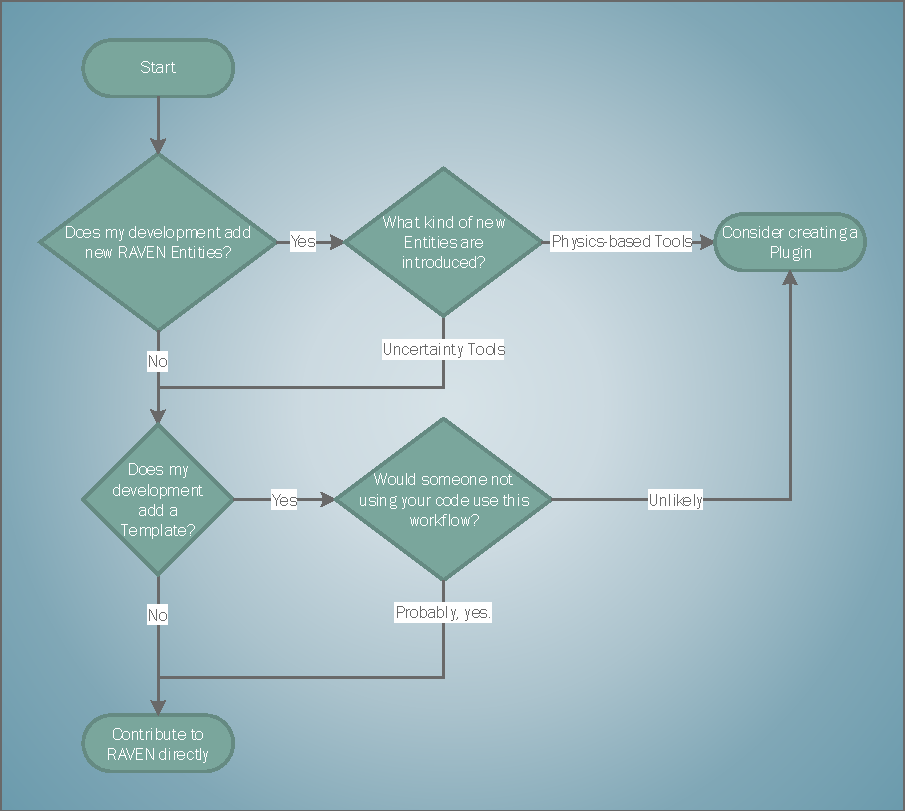
\includegraphics[scale=0.7]{pics/toPluginOrNot.pdf}
  \caption{Choosing to Plugin Workflow}
  \label{fig:choose plugin}
 \end{figure}

 \subsection{Supported Plugins}

 Officially supported RAVEN Plugins are a subset of all Plugins filtered by a particular set of characteristics. It is intended that all official Plugins are compatible with the latest developments in RAVEN as well as with each other. Additionally, official plugins contain continuous integration (CI) testing and provide the necessary software quality assurance (SQA) documentation to be included in RAVEN's SQA plan.

 To be an officially supported RAVEN Plugin, the following prerequesites must be met:
 \begin{itemize}
  \item The appropriate SQA documentation for NQA-1 level 2 coverage under the RAVEN SQA must be in place for the Plugin.
  \item The Plugin must contain CI testing with coverage consistent with RAVEN SQA. This CI testing must be compatible with RAVEN's CI testing system.
  \item The Plugin must contain documentation explaining the use and options included in the Plugin's contents.
  \item If at any time a change in RAVEN causes a failure in the CI tests in the plugin, the plugin must be updated to be compatible with the new RAVEN.
 \end{itemize}

 If a Plugin fails any of these criteria, a grace period (usually a month) is provided along with
 notification to the Plugin developers. If the grace period expires and the Plugin does not meet the
 requirements, it may be removed from the official supported Plugins list, pending an update to the
 Plugin.


\input{ravenTutorial.tex}
\section{Forward Sampling Strategies}
\label{sec:forwardSamplingStrategies}
In order to perform UQ and dynamic
probabilistic risk assessment (DPRA),
a sampling strategy needs to be employed. The sampling strategy
perturbs the input space (domain of the uncertainties) to explore
the response of a complex system in relation to selected FOMs.

The most widely used strategies to perform UQ and PRA are generally
collected in RAVEN as \textit{\textbf{Forward}} samplers. \textit{\textbf{Forward}} samplers include
all the strategies that simply perform the sampling of the input space.  These strategies sample
without exploiting, through learning approaches,
the information made available from the outcomes of evaluation previously performed (adaptive sampling) and the
common system evolution (patterns) that different sampled calculations can generate in the phase space (Dynamic Event Tree).

As mentioned in Section~\ref{sub:tutorialMultiRun}, RAVEN has
several different \textit{\textbf{Forward}} samplers:
\begin{itemize}
  \item \textit{Monte-Carlo}
  \item \textit{Grid-based}
  \item \textit{Stratified} and its specialization named \textit{Latin Hyper Cube}.
\end{itemize}
In addition, RAVEN posses advanced \textit{\textbf{Forward}} sampling strategies that:
\begin{itemize}
  \item Build a grid in the input space selecting evaluation points
    based on characteristic quadratures as part of stochastic collocation
    for generalized polynomial chaos method (\textit{Sparse
    Grid Collocation} sampler);
  \item Use high-density model reduction (HDMR) a.k.a. Sobol
    decomposition to approximate a function as the sum of
    interactions with increasing complexity (\textit{Sobol} sampler).
\end{itemize}
In the following subsections, we provide examples of input files
in RAVEN using the method, with explanatory commentary.
%%%%%%%%%%%%%%%%%%%%%%%%%
%%%%%%%%  MONTE-CARLO %%%%%%%%
%%%%%%%%%%%%%%%%%%%%%%%%%
\subsection{Monte-Carlo sampling through RAVEN}
\label{sub:MCexample}
The Monte-Carlo method is one of the most-used methodologies in several mathematic disciplines. In this section,
we will explain the techniques for employing this methodology in RAVEN, and we recommend the user to read the
theory manual to explore the theory of the method.
The goals of this section are about learning how to:
 \begin{enumerate}
   \item Set up a simple Monte-Carlo sampling for perturbing the input space of a driven code
   \item Load the outputs of the code into RAVEN DataObjects (HistorySets and PointSets)
   \item Print the contents of DataObjects to file
   \item Generate plots of the sampling results.
\end{enumerate}
In order to accomplish these tasks, the following RAVEN \textbf{Entities} (XML blocks in the RAVEN input file) are needed:
\begin{enumerate}
   \item \textbf{\textit{RunInfo}}:
     \xmlExample{framework/user_guide/ForwardSamplingStrategies/forwardSamplingMontecarlo.xml}{RunInfo}
     As discussed in Section~\ref{sub:singleRun}, the \textit{RunInfo} \textbf{Entity} sets up the analysis
     that the user wants to perform. The number of steps specified in (\xmlNode{Sequence}) are sequentially run using the number of processors assigned in (\xmlNode{batchSize}). 
     Note that the \xmlNode{JobName} is not required, but is useful in identifying the input file.
   \item \textbf{\textit{Models}}:
     \xmlExample{framework/user_guide/ForwardSamplingStrategies/forwardSamplingMontecarlo.xml}{Models}
     The Model used in this example is the \textbf{Projectile} external model, which is defined in section \ref{sec:analyticalbateman}.  
   \item \textbf{\textit{Distributions}}:
     \xmlExample{framework/user_guide/ForwardSamplingStrategies/forwardSamplingMontecarlo.xml}{Distributions}
     In the \xmlNode{Distributions} block, the stochastic model for the uncertainties treated by the
     \xmlNode{Sampler} is defined. In this case two distributions are defined:
  \begin{itemize}
    \item $vel\_dist \sim \mathbb{N}(30,5)$, used to model the uncertainties
    associated with  the \textit{velocity};
    \item  $angle\_dist \sim \mathbb{U}(5,85)$,  used to
    model the uncertainties associated with the \textit{angle}.
  \end{itemize}
   \item \textbf{\textit{Samplers}}:
     \xmlExample{framework/user_guide/ForwardSamplingStrategies/forwardSamplingMontecarlo.xml}{Samplers}
      To employ the Monte-Carlo sampling strategy, a
      \xmlNode{MonteCarlo} node needs to be defined. The number of samples is defined within this node. The Monte-Carlo method is employed on model variables listed by name and are associated with a distribution.
   \item \textbf{\textit{DataObjects}}:
     \xmlExample{framework/user_guide/ForwardSamplingStrategies/forwardSamplingMontecarlo.xml}{DataObjects}
      In this block, three \textit{DataObjects} are defined to store results: 1) a PointSet named
      ``samples'', 2) a PointSet named ``dummyIN'' 3) a HistorySet named ``histories''.
      Note that in the \xmlNode{Input} node all the uncertainties
      perturbed through the Monte-Carlo strategy are listed. By this, any
      realization in the input space is linked in the DataObject to the outputs listed in the
      \xmlNode{Output} node. Furthermore, since we use an external model that does not have any input file, we define a pointset named ``dummyIN'' that is used as a dummy input in the multirun step.
   \item \textbf{\textit{OutStreams}}:
     \xmlExample{framework/user_guide/ForwardSamplingStrategies/forwardSamplingMontecarlo.xml}{OutStreams}
 %%%%%%%%%%%%%%%%%%%%%%%%%%%%%%%%%%%%%%%%%%%%%%%%%%%%%%%%%%
 %figure histories
 \begin{figure}[h!]
  \centering
  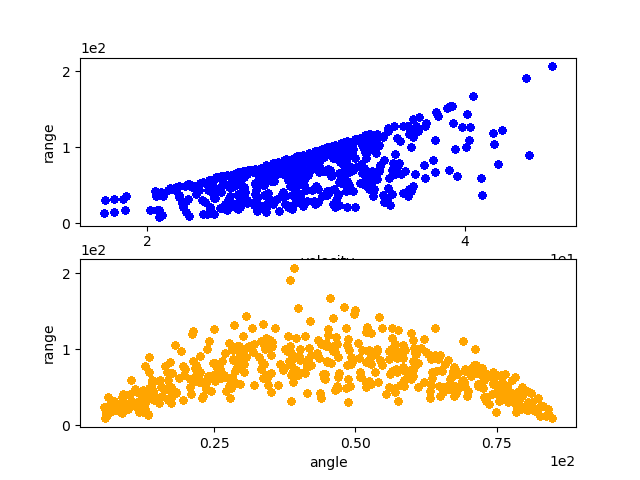
\includegraphics[scale=0.7]{../../tests/framework/user_guide/ForwardSamplingStrategies/gold/RunDir/MonteCarlo/1-historyPlot_scatter-scatter.png}
  \caption{Plot of the histories generated by the Monte Carlo sampling.}
  \label{fig:historiesMCPlotScatter}
 \end{figure}
 %%%%%%%%%%%%%%%%%%%%%%%%%%%%%%%%%%%%%%%%%%%%%%%%%%%%%%%%%%
 To see the results of the simulation, \xmlNode{OutStreams} are included in the input.
  In this block, both OutStream types are used:
  \begin{itemize}
    \item \textit{Print}:
     \begin{itemize}
       \item ``samples'' connected with the \textit{DataObjects} \textbf{Entity} ``samples''
                (\xmlNode{source})
       \item ``histories'' connected with the \textit{DataObjects} \textbf{Entity} ``histories'' (\xmlNode{source})
     \end{itemize}
     Note that in RAVEN, multiple entities can have the same name, as it takes a class, a type, and a name to uniquely identify a RAVEN object. When the two OutStream objects are used, all the information contained in the  linked \textit{DataObjects} are going
    to be exported in CSV files (\xmlNode{type}).
    \item \textit{Plot}:
    \begin{itemize}
      \item ``historiesPlot'' connected with the  \textit{DataObjects}
      \textbf{Entity} ``histories''.  This plot shows the variable $range$ with respect to the input variables $velocity$ and $angle$.
      \item ``samplesPlot3D'' connected with the
      \textit{DataObjects} \textbf{Entity} ``samples''. This plot shows the variables $range,time$ with respect to the input variables $velocity$ and $angle$.
    \end{itemize}
     Note that both plots use gridded subplots. Two plots
     are placed in each of the figures.
  \end{itemize}
   \item \textbf{\textit{Steps}}:
     \xmlExample{framework/user_guide/ForwardSamplingStrategies/forwardSamplingMontecarlo.xml}{Steps}
 %%%%%%%%%%%%%%%%%%%%%%%%%%%%%%%%%%%%%%%%%%%%%%%%%%%%%%%%%%
 %figure samples
 \begin{figure}[h!]
  \centering
  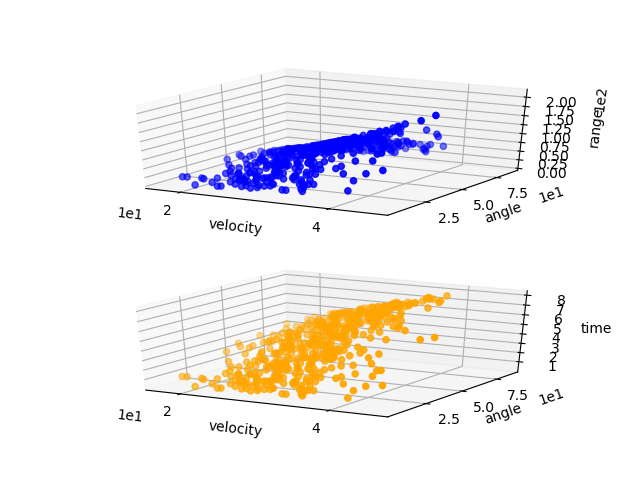
\includegraphics[scale=0.7]{../../tests/framework/user_guide/ForwardSamplingStrategies/gold/RunDir/MonteCarlo/1-samplesPlot3D_scatter-scatter.png}
  \caption{Plot of the samples generated by the MC sampling.}
  \label{fig:samplesMCPlotScatter}
 \end{figure}
 %%%%%%%%%%%%%%%%%%%%%%%%%%%%%%%%%%%%%%%%%%%%%%%%%%%%%%%%%%
   Once all the other entities are defined in the RAVEN input file, they must be combined in the
   \xmlNode{Steps} block, which dictates the workflow of RAVEN.  For this case,
   two \xmlNode{Steps} are defined:
   \begin{itemize}
     \item \xmlNode{MultiRun} ``sample'', used to run the multiple
     instances of the driven code and
     collect the outputs in the two \textit{DataObjects}. As it can be
     seen, the \xmlNode{Sampler} is specified to communicate to the
     \textit{Step} that the driven code needs to
     be perturbed through the Monte-Carlo sampling.
     \item  \xmlNode{IOStep} named ``writeHistories'', used to 1) dump
     the ``histories'' and ``samples'' \textit{DataObjects}
     \textbf{Entity} to a CSV file and 2) plot the data in the EPS file.
   \end{itemize}
\end{enumerate}
 Figures~\ref{fig:historiesMCPlotScatter} and ~\ref{fig:samplesMCPlotScatter} show the report
 generated by RAVEN.
%%%%%%%%%%%%%%%%%%%%%%%%%
%%%%%%%%          GRID          %%%%%%%%
%%%%%%%%%%%%%%%%%%%%%%%%%
\subsection{Grid sampling through RAVEN}
\label{sub:Gridexample}
The Grid sampling method (also known as Full Factorial Design of Experiment) represents one of the simplest methodologies that can be employed in order to explore the interaction of multiple random variables with respect
selected FOMs.
The goal of this section is to show how to:
 \begin{enumerate}
   \item Set up a simple Grid sampling for performing a parametric analysis of a driven code
   \item Load the outputs of the code into the RAVEN DataObjects system
   \item Print out what contained in the DataObjects
   \item Generate basic plots of the code result.
\end{enumerate}
In order to accomplish these tasks, the following RAVEN \textbf{Entities} (XML blocks in the input files) are required:
\begin{enumerate}
   \item \textbf{\textit{RunInfo}}:
     \xmlExample{framework/user_guide/ForwardSamplingStrategies/forwardSamplingGrid.xml}{RunInfo}
   As shown in Section~\ref{sub:singleRun}, the \textit{RunInfo} \textbf{Entity} is intended to set up the desired analysis. The number of steps specified in (\xmlNode{Sequence}) are sequentially run using the number of processors assigned in (\xmlNode{batchSize}). 
   \item \textbf{\textit{Models}}:
     \xmlExample{framework/user_guide/ForwardSamplingStrategies/forwardSamplingGrid.xml}{Models}
 The Model here is represented by the \textbf{Projectile}, which already dumps its output file in a
 CSV format (standard format that RAVEN can read). 
   \item \textbf{\textit{Distributions}}:
     \xmlExample{framework/user_guide/ForwardSamplingStrategies/forwardSamplingGrid.xml}{Distributions}
  In the Distributions XML section, the stochastic model for the
  uncertainties  treated by the Grid sampling are reported. In
  this case two distributions are defined:
  \begin{itemize}
    \item $vel\_dist \sim \mathbb{N}(30,5)$, used to model the uncertainties
    associated with  the \textit{velocity};
    \item  $angle\_dist \sim \mathbb{U}(5,85)$,  used to
    model the uncertainties associated with the \textit{angle}.
  \end{itemize}
   \item \textbf{\textit{Samplers}}:
     \xmlExample{framework/user_guide/ForwardSamplingStrategies/forwardSamplingGrid.xml}{Samplers}
  To employ the Grid sampling strategy, a
  \xmlNode{Grid} node needs to be specified. As shown above, in each variable section, the  \xmlNode{grid} is defined.
   \item \textbf{\textit{DataObjects}}:
     \xmlExample{framework/user_guide/ForwardSamplingStrategies/forwardSamplingGrid.xml}{DataObjects}
  In this block, three \textit{DataObjects} are defined to store results: 1) a PointSet named
      ``samples'', 2) a PointSet named ``dummyIN'' 3) a HistorySet named ``histories''.
  In the \xmlNode{Input} node all the variables  perturbed through the Grid strategy are listed. In this way, any  realization in the input space is linked to the outputs listed in  the
  \xmlNode{Output} node. As described earlier as well, since we use an external model that does not have any input file, we define a pointset named ``dummyIN'' that is used as a dummy input in the multirun step.
    \item \textbf{\textit{OutStreams}}:
     \xmlExample{framework/user_guide/ForwardSamplingStrategies/forwardSamplingGrid.xml}{OutStreams}
 %%%%%%%%%%%%%%%%%%%%%%%%%%%%%%%%%%%%%%%%%%%%%%%%%%%%%%%%%%
 %figure histories
 \begin{figure}[h!]
  \centering
  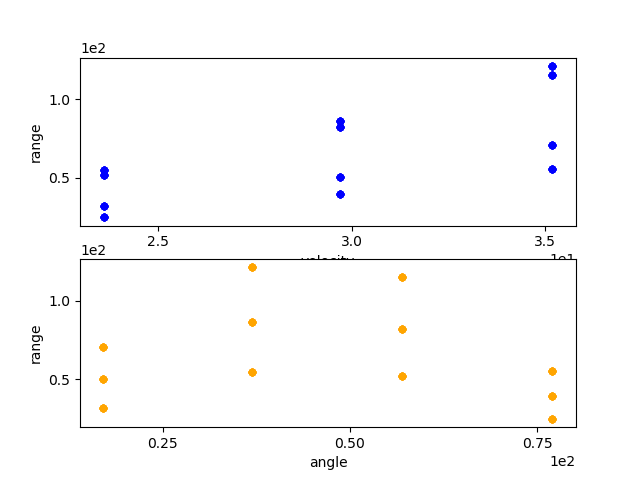
\includegraphics[scale=0.7]{../../tests/framework/user_guide/ForwardSamplingStrategies/gold/RunDir/Grid/1-historyPlot_scatter-scatter.png}
  \caption{Plot of the histories generated by the Grid sampling.}
  \label{fig:historiesGridPlotScatter}
 \end{figure}
 %%%%%%%%%%%%%%%%%%%%%%%%%%%%%%%%%%%%%%%%%%%%%%%%%%%%%%%%%%
  In this block, both the Out-Stream types are constructed:
  \begin{itemize}
    \item \textit{Print}:
     \begin{itemize}
       \item named ``samples'' connected with the \textit{DataObjects} \textbf{Entity} ``samples''
                (\xmlNode{source})
       \item named ``histories'' connected with the \textit{DataObjects} \textbf{Entity} ``histories'' (\xmlNode{source}).
     \end{itemize}
      When these objects get used, all the information contained in the
      linked  \textit{DataObjects} are going
    to be exported in CSV files (\xmlNode{type}).
    \item \textit{Plot}:
    \begin{itemize}
      \item named ``historiesPlot'' connected with the  \textit{DataObjects}
      \textbf{Entity} ``histories''.  This plot shows the variable $range$ with respect to the input variables $velocity$ and $angle$.
      \item named ``samplesPlot3D'' connected with the
      \textit{DataObjects} \textbf{Entity} ``samples''. This plot shows the variables $range,time$ with respect to the input variables $velocity$ and $angle$.
    \end{itemize}
  \end{itemize}
   \item \textbf{\textit{Steps}}:
     \xmlExample{framework/user_guide/ForwardSamplingStrategies/forwardSamplingGrid.xml}{Steps}
 %%%%%%%%%%%%%%%%%%%%%%%%%%%%%%%%%%%%%%%%%%%%%%%%%%%%%%%%%%
 %figure samples
 \begin{figure}[h!]
  \centering
  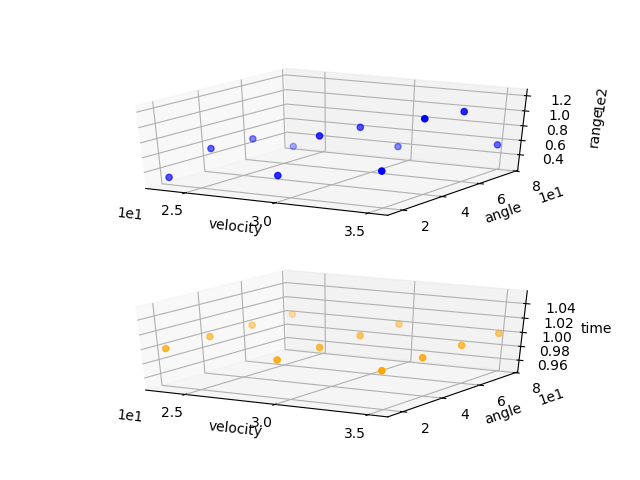
\includegraphics[scale=0.7]{../../tests/framework/user_guide/ForwardSamplingStrategies/gold/RunDir/Grid/1-samplesPlot3D_scatter-scatter.png}
  \caption{Plot of the samples generated by the Grid sampling for variables $A,B,C,D$.}
  \label{fig:samplesGridPlotScatter}
 \end{figure}
 %%%%%%%%%%%%%%%%%%%%%%%%%%%%%%%%%%%%%%%%%%%%%%%%%%%%%%%%%%
   Finally, all the previously defined \textbf{Entities} can be combined in
   the \xmlNode{Steps} block. As inferable,
   two \xmlNode{Steps} have been inputted:
   \begin{itemize}
     \item \xmlNode{MultiRun} named ``sample'', is used to run the multiple
     instances of the code and
     collect the outputs in the two \textit{DataObjects}. As it can be
     seen, the \xmlNode{Sampler} is inputted to communicate to the
     \textit{Step} that the driven code needs to
     be perturbed through the Grid sampling
     \item  \xmlNode{IOStep} named ``writeHistories'', used to 1) dump
     the ``histories'' and ``samples'' \textit{DataObjects}
     \textbf{Entity} in a CSV file and 2) plot the data in the PNG file and
     on the screen.
   \end{itemize}
\end{enumerate}
 Figures~\ref{fig:historiesGridPlotScatter} and ~\ref{fig:samplesGridPlotScatter} display the report generated by RAVEN.

%%%%%%%%%%%%%%%%%%%%%%%%%
%%%%%%%%    STRATIFIED    %%%%%%%%
%%%%%%%%%%%%%%%%%%%%%%%%%
\subsection{Stratified sampling through RAVEN}
\label{sub:Stratifiedexample}
The Stratified sampling is a class of methods that relies on the assumption that the input space (i.e.,uncertainties)
can be separated in regions (strata) based on similarity of the response of the system for input set within the
same strata. Following this assumption, the most rewarding (in terms of computational cost vs. knowledge gain)
sampling strategy would be to place one sample for each region. In this way, the same information is not
collected more than once and all the prototypical behavior are sampled at least once. In
Figure~\ref{fig:StratifiedSamplingExample}, the Stratified sampling approach is exemplified.
 \begin{figure}[h!]
  \centering
  \includegraphics[scale=0.55]{pics/StratifiedSamplingExample.png}
  \caption{Example of Stratified sampling approach.}
  \label{fig:StratifiedSamplingExample}
 \end{figure}
\\The goal of this section is to show how to:
 \begin{enumerate}
   \item Set up a simple Stratified sampling in order to perform a parametric analysis on a driven code
   \item Load the outputs of the code into the RAVEN DataObjects system
   \item Print out what contained in the DataObjects
   \item Generate basic plots of the code result.
\end{enumerate}
To accomplish these tasks, the following RAVEN \textbf{Entities} (XML blocks in the input files) are defined:
\begin{enumerate}
   \item \textbf{\textit{RunInfo}}:
     \xmlExample{framework/user_guide/ForwardSamplingStrategies/forwardSamplingStratified.xml}{RunInfo}
   As explained earlier, the \textit{RunInfo} \textbf{Entity} is intended to set up the analysis that the user wants to perform. The number of steps specified in (\xmlNode{Sequence}) are sequentially run using the number of processors assigned in (\xmlNode{batchSize}).
   \item \textbf{\textit{Models}}:
     \xmlExample{framework/user_guide/ForwardSamplingStrategies/forwardSamplingStratified.xml}{Models}
 The Model here is represented by the
 \textbf{Projectile}, which already dumps its output file in a
 CSV format (standard format that RAVEN can read).
   \item \textbf{\textit{Distributions}}:
     \xmlExample{framework/user_guide/ForwardSamplingStrategies/forwardSamplingStratified.xml}{Distributions}
  In the Distributions XML section, the stochastic model for the
  uncertainties  treated by the Stratified sampling are reported. In
  this case two distributions are defined:
  \begin{itemize}
    \item $vel\_dist \sim \mathbb{N}(30,5)$, used to model the uncertainties
    associated with  the \textit{velocity};
    \item  $angle\_dist \sim \mathbb{U}(5,85)$,  used to
    model the uncertainties associated with the \textit{angle}.
  \end{itemize}
   \item \textbf{\textit{Samplers}}:
     \xmlExample{framework/user_guide/ForwardSamplingStrategies/forwardSamplingStratified.xml}{Samplers}
  To employ the Stratified sampling strategy, a
  \xmlNode{Stratified} node needs to be specified. In each variable section, the  \xmlNode{grid} is defined.
  It is important to mention that the number of \xmlAttr{steps} needs to be the same for each of the variables,  since, as reported in previous section, the Stratified sampling strategy it discretizes the domain in strata.
  The number of samples finally requested is equal to $n_{samples} = n_{steps} = 100$.
  If the grid for each variables is defined in CDF and of  \xmlAttr{type} = ``equal'', the Stratified sampling corresponds to the well-known Latin Hyper Cube sampling.
   \item \textbf{\textit{DataObjects}}:
     \xmlExample{framework/user_guide/ForwardSamplingStrategies/forwardSamplingStratified.xml}{DataObjects}
  In this block, two \textit{DataObjects} are defined: 1) a PointSet named
      ``samples'', 2) a PointSet named ``dummyIN'' 3) a HistorySet named ``histories''.
  In the \xmlNode{Input} node all the variables perturbed through the Stratified strategy are listed. In this way, any realization in the input space is linked to the outputs listed in  the
  \xmlNode{Output} node. Since we use an external model that does not have any input file, we define a pointset named ``dummyIN'' that is used as a dummy input in the multirun step.
   \item \textbf{\textit{OutStreams}}:
     \xmlExample{framework/user_guide/ForwardSamplingStrategies/forwardSamplingStratified.xml}{OutStreams}
 %%%%%%%%%%%%%%%%%%%%%%%%%%%%%%%%%%%%%%%%%%%%%%%%%%%%%%%%%%
 %figure histories
 \begin{figure}[h!]
  \centering
  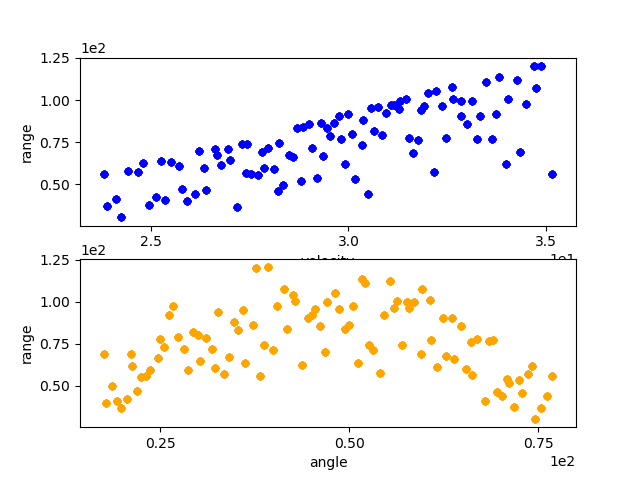
\includegraphics[scale=0.7]{../../tests/framework/user_guide/ForwardSamplingStrategies/gold/RunDir/Stratified/1-historyPlot_scatter-scatter.png}
  \caption{Plot of the histories generated by the Stratified sampling.}
  \label{fig:historiesStratifiedPlotScatter}
 \end{figure}
 %%%%%%%%%%%%%%%%%%%%%%%%%%%%%%%%%%%%%%%%%%%%%%%%%%%%%%%%%%
  In this block, both the Out-Stream types are constructed:
  \begin{itemize}
    \item \textit{Print}:
     \begin{itemize}
       \item named ``samples'' connected with the \textit{DataObjects} \textbf{Entity} ``samples''
                (\xmlNode{source})
       \item named ``histories'' connected with the \textit{DataObjects} \textbf{Entity} ``histories'' (\xmlNode{source}).
     \end{itemize}
      When these objects get used, all the information contained in the
      linked  \textit{DataObjects} are going
    to be exported in CSV files (\xmlNode{type}).
    \item \textit{Plot}:
    \begin{itemize}
      \item named ``historiesPlot'' connected with the  \textit{DataObjects}
      \textbf{Entity} ``histories''.  This plot shows the variable $range$ with respect to the input variables $velocity$ and $angle$.
      \item named ``samplesPlot3D'' connected with the
      \textit{DataObjects} \textbf{Entity} ``samples''. This plot shows the variables $range,time$ with respect to the input variables $velocity$ and $angle$.
    \end{itemize}
  \end{itemize}
   \item \textbf{\textit{Steps}}:
     \xmlExample{framework/user_guide/ForwardSamplingStrategies/forwardSamplingStratified.xml}{Steps}
 %%%%%%%%%%%%%%%%%%%%%%%%%%%%%%%%%%%%%%%%%%%%%%%%%%%%%%%%%%
 %figure samples
 \begin{figure}[h!]
  \centering
  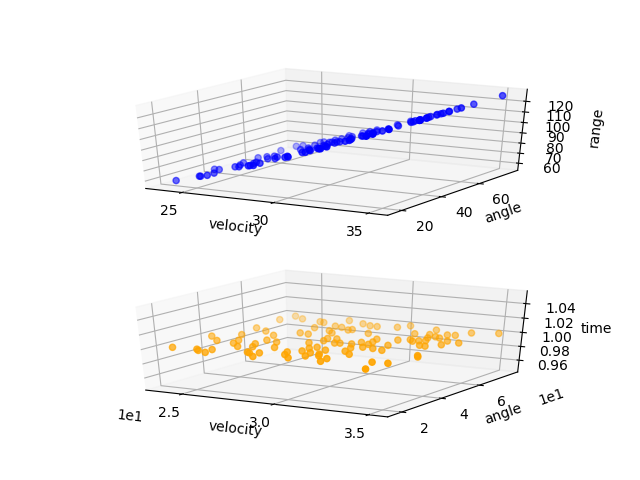
\includegraphics[scale=0.7]{../../tests/framework/user_guide/ForwardSamplingStrategies/gold/RunDir/Stratified/1-samplesPlot3D_scatter-scatter.png}
  \caption{Plot of the samples generated by the Stratified sampling.}
  \label{fig:samplesStratifiedPlotLine}
 \end{figure}
 %%%%%%%%%%%%%%%%%%%%%%%%%%%%%%%%%%%%%%%%%%%%%%%%%%%%%%%%%%
   Finally, all the previously defined \textbf{Entities} can be combined in
   the \xmlNode{Steps} block. As inferable,
   two \xmlNode{Steps} have been inputted:
   \begin{itemize}
     \item \xmlNode{MultiRun} named ``sample'', used to run the multiple
     instances of the driven code and
     collect the outputs in the two \textit{DataObjects}. As it can be
     seen, the \xmlNode{Sampler} is inputted to communicate to the
     \textit{Step} that the driven code needs to
     be perturbed through the Stratified sampling.
     \item  \xmlNode{IOStep} named ``writeHistories'', used to 1) dump
     the ``histories'' and ``samples'' \textit{DataObjects}
     \textbf{Entity} in a CSV file and 2) plot the data in the PNG file and
     on the screen.
   \end{itemize}
\end{enumerate}
 As previously mentioned, Figures~\ref{fig:historiesStratifiedPlotScatter} and ~\ref{fig:samplesStratifiedPlotScatter}  display the report generated by RAVEN.

%%%%%%%%%%%%%%%%%%%%%%%%%

\subsection{Sparse Grid Collocation sampling through RAVEN}
\label{sub:SGcsamplingExample}
The Sparse Grid Collocation sampler represents an advanced methodology to perform Uncertainty Quantification. They aim
to explore the input space leveraging the information contained in the associated probability density functions. It builds on generic Grid sampling by selecting evaluation points based on characteristic quadratures as part of stochastic collocation for generalized polynomial chaos uncertainty quantification. In collocation an N-D grid is constructed, with each uncertain variable providing an axis. Along each axis, the points of evaluation correspond to quadrature points necessary to integrate polynomials. In the simplest (and most naive) case, a N-D tensor product of all possible combinations of points from each dimension’s quadrature is constructed as sampling points. The number of necessary samples can be reduced by employing Smolyak-like sparse grid algorithms, which use reduced combinations of polynomial orders to reduce the necessary sampling space.
\\The goals of this section are about learning how to:
 \begin{enumerate}
   \item Set up a Sparse Grid Collocation sampling for the construction of a suitable surrogate model of a driven code
   \item Construct a GaussPolynomialRom surrogate model (training stage)
   \item Use the constructed GaussPolynomialRom surrogate model instead of the driven code.
\end{enumerate}
To accomplish these tasks, the following RAVEN \textbf{Entities} (XML blocks in the input files) need to be defined:
\begin{enumerate}
   \item \textbf{\textit{RunInfo}}:
     \xmlExample{framework/user_guide/ForwardSamplingStrategies/forwardSamplingSparseGrid.xml}{RunInfo}
   AThe \textit{RunInfo} \textbf{Entity} is intended to set up the analysis  that the user wants to perform. The steps listed in (\xmlNode{Sequence}) are going to be sequentially run using the number of processors specified in  (\xmlNode{batchSize}).  The first two steps build the ROM
   (\xmlString{sample}, \xmlString{train}), the next two validate
   the ROM against the original Code Model (\xmlString{validateModel}, \xmlString{validateROM}),
   \xmlString{rom\_stats} stores ROM-related information into DataObject,
   and the last two produce plots and print data (\xmlString{output\_print}, \xmlString{output\_plot}).
   \item \textbf{\textit{Models}}:
     \xmlExample{framework/user_guide/ForwardSamplingStrategies/forwardSamplingSparseGrid.xml}{Models}
 The goal of this example is the generation of a \text{GaussPolynomialRom}
 for subsequent usage.  In addition to the previously explained External model, the ROM of type \textit{GaussPolynomialRom} is specified here. The ROM is generated through a Sparse Grid Collocation sampling strategy. Note that the \xmlNode{Interpolation} nodes are not required, but are included for the sake of demonstration.
   \item \textbf{\textit{Distributions}}:
     \xmlExample{framework/user_guide/ForwardSamplingStrategies/forwardSamplingSparseGrid.xml}{Distributions}
  In the Distributions XML section, the stochastic model for the
  uncertainties  treated by the Sparse Grid Collocation sampling are reported. In
  this case two distributions are defined:
  \begin{itemize}
    \item $vel\_dist \sim \mathbb{N}(30,5)$, used to model the uncertainties
    associated with  the \textit{velocity};
    \item  $angle\_dist \sim \mathbb{U}(5,85)$,  used to
    model the uncertainties associated with the \textit{angle}.
  \end{itemize}
   \item \textbf{\textit{Samplers}}:
     \xmlExample[rom,ROM,SparseGridCollocation,MonteCarlo]{framework/user_guide/ForwardSamplingStrategies/forwardSamplingSparseGrid.xml}{Samplers}
  In order to employ the Sparse Grid Collocation sampling strategy, a
  \xmlNode{SparseGridCollocation} node needs to be defined.
  As can be  seen from above, each variable is associated with a different distribution,
  defined in the  \xmlNode{Distributions} block.
  In addition, the \textit{GaussPolynomialRom} \xmlNode{ROM} is linked to the \xmlNode{SparseGridCollocation} sampler.  Because this sampler is used exclusively to build the ROM, some of the parameters of the ROM are  needed by the sampler, and this connection makes that communication possible.  The setting of this ROM (e.g. polynomial order, Index set method, etc.) determines how the Stochastic Collocation Method is employed.

  Additionally, a \xmlNode{MonteCarlo} sampler is set up for validating the ROM against the original Code.  The random number generation seed (\xmlNode{initialSeed}) is specified and set to reset on each use (\xmlNode{reseedEachIteration}) so that the Monte Carlo sampler can be used to compare the ROM against the  original model.  We use 100 samples (\xmlNode{limit}) to sample the ROM and the model, and then print and plot both data sets to compare them.
   \item \textbf{\textit{DataObjects}}:
     \xmlExample[rom,SparseGridCollocation]{framework/user_guide/ForwardSamplingStrategies/forwardSamplingSparseGrid.xml}{DataObjects}
  In this block, five \textit{DataObjects} are defined:
  1) a PointSet named ``inputPlaceholder'' used as a placeholder input for the ROM sampling step,
  2) a PointSet named ``samplesModel'' to store the Code responses from Monte Carlo samples,
  3) a PointSet named ``samplesROM'' to store the ROM responses from Monte Carlo samples,
  4) a HistorySet named ``histories'' used to collect the samples needed to train the ROM, and
  5) a DataSet named ``rom\_stats'' to store information from the ROM.
 %%%%%%%%%%%%%%%%%%%%%%%%%%%%%%%%%%%%%%%%%%%%%%%%%%%%%%%%%%
 %%%%%%%%%%%%%%%%%%%%%%%%%%%%%%%%%%%%%%%%%%%%%%%%%%%%%%%%%%
 %figure histories
 \begin{figure}[h!]
  \centering
  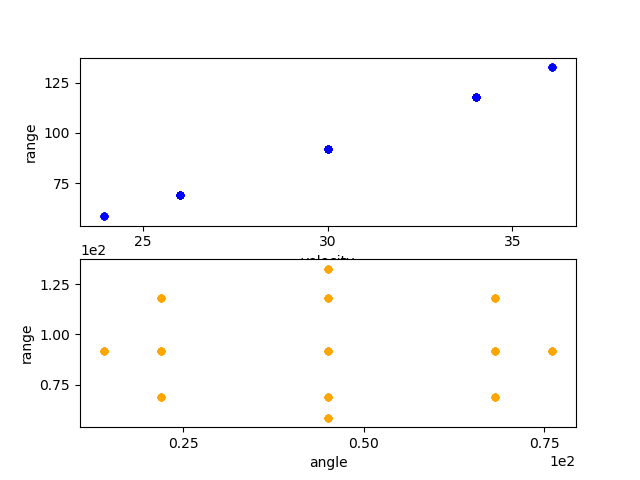
\includegraphics[scale=0.7]{../../tests/framework/user_guide/ForwardSamplingStrategies/gold/RunDir/SparseGrid/1-historyPlot_scatter-scatter.png}
  \caption{Plot of the training samples generated by the SparseGridCollocation sampling for variables $A,B,C,D$.}
  \label{fig:historiesSparseGridPlotScatter}
 \end{figure}
 %%%%%%%%%%%%%%%%%%%%%%%%%%%%%%%%%%%%%%%%%%%%%%%%%%%%%%%%%%
 %%%%%%%%%%%%%%%%%%%%%%%%%%%%%%%%%%%%%%%%%%%%%%%%%%%%%%%%%%
   \item \textbf{\textit{OutStreams}}:
     \xmlExample{framework/user_guide/ForwardSamplingStrategies/forwardSamplingSparseGrid.xml}{OutStreams}
  In this block, the following Out-Stream types are constructed:
  \begin{itemize}
    \item \textit{Print}:
     \begin{itemize}
       \item named ``samplesModel'' connected with the \textit{DataObjects} \textbf{Entity} ``samplesModel''
                (\xmlNode{source})
       \item named ``samplesROM'' connected with the \textit{DataObjects} \textbf{Entity} ``samplesROM''
                (\xmlNode{source})
       \item named ``histories'' connected with the \textit{DataObjects} \textbf{Entity} ``histories'' (\xmlNode{source})
       \item named ``rom\_output'' connected with the \textit{ROM} \textbf{Entity} ``rom'' (\xmlNode{source}).
     \end{itemize}
      When these objects get used, all the information contained in the
      linked  \textit{DataObjects} are going
    to be exported in ether CSV files for DataObjects or XML files for ROMs (\xmlNode{type}).
    \item \textit{Plot}:
    \begin{itemize}
      \item named ``historyPlot'' connected with the  \textit{DataObjects}
      \textbf{Entity} ``histories''.  This plots the
      variable $range$ with respect to the input variables $velocity$ and $angle$.
      \item named ``samplesModelPlot3D'' connected with the
      \textit{DataObjects} \textbf{Entity} ``samplesModel''. This plot will draw the
      variables $range,time$ as Monte Carlo sampled on the Code.
      \item named ``samplesROMPlot3D'' connected with the
      \textit{DataObjects} \textbf{Entity} ``samplesROM''. This plot will draw the
      variables $range,time$ as Monte Carlo sampled on the ROM.
    \end{itemize}
  \end{itemize}
   \item \textbf{\textit{Steps}}:
     \xmlExample[rom,SparseGridCollocation]{framework/user_guide/ForwardSamplingStrategies/forwardSamplingSparseGrid.xml}{Steps}
  %%%%%%%%%%%%%%%%%%%%%%%%%%%%%%%%%%%%%%%%%%%%%%%%%%%%%%%%%%
 %figure samples
 \begin{figure}[h!]
  \centering
  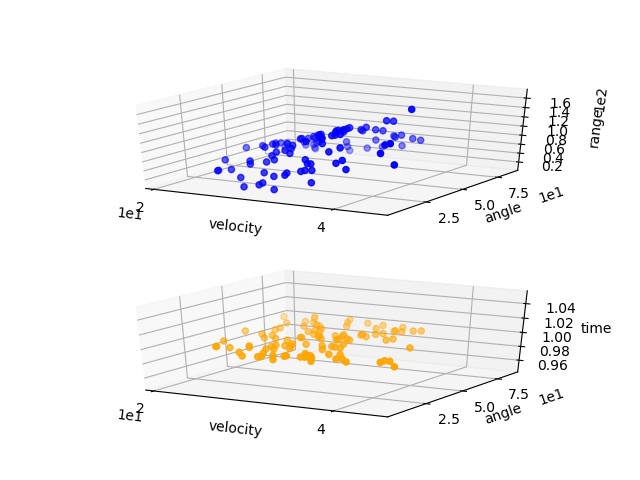
\includegraphics[scale=0.7]{../../tests/framework/user_guide/ForwardSamplingStrategies/gold/RunDir/SparseGrid/1-samplesModelPlot3D_scatter-scatter.png}
  \caption{Plot of validation samples generated by Monte Carlo sampling on the Code.}
  \label{fig:samplesSparseGridPlotModel}
 \end{figure}
 %%%%%%%%%%%%%%%%%%%%%%%%%%%%%%%%%%%%%%%%%%%%%%%%%%%%%%%%%%
   Finally, the previously defined \textbf{Entities} can be combined in
   the \xmlNode{Steps} block.
   The following \xmlNode{Steps} have been defined:
   \begin{itemize}
     \item \xmlNode{MultiRun} named ``sample'', used to run the training
     samples of the driven code and
     collect the outputs in the \textit{DataObjects}.
     The \xmlNode{Sampler} is specified to communicate to the
     \textit{Step} that the driven code needs to
     be sampled through the Sparse Grid Collocation sampling strategy;
     \item \xmlNode{RomTrainer} named ``train'', used to train (i.e.,
     construct) the GaussPolynomial ROM. This step is essential if the
     user want to use the ROM in later steps;
     \item \xmlNode{MultiRun} named ``sampleModel'', used to run the
     Monte Carlo perturbed samples of the original Model for use in verification.  The results are
     collected in the \textit{samplesModel} \textit{DataObjects}.
     \item \xmlNode{MultiRun} named ``sampleROM'', used to run the
     Monte Carlo perturbed samples of the previously constructed ROM for use in verificaiton.  The results are
     collected in the \textit{samplesROM} \textit{DataObjects}.
     \item \xmlNode{IOStep} named ``rom\_stas'', used to dump rom-related information into \textit{DataObject },
     \item  \xmlNode{IOStep} named ``output\_print'', used to dump
     the ``histories'', ``samplesModel'' and ``samplesROM'' \textit{DataObjects}
     \textbf{Entity} in a CSV file,
     \item  \xmlNode{IOStep} named ``output\_plot'', used to
     plot the data and store it in the PNG file and
     on the screen.
   \end{itemize}
\end{enumerate}
 % As previously mentioned, Figure~\ref{fig:historiesSparseGridPlotScatter}
 % shows the evolution of the outputs $A,B,C,D$ under uncertainties.
 % Figures~\ref{fig:samplesSparseGridPlotModel} and
 % \ref{fig:samplesROMSparseGridPlot} show the final responses
 % of the sampling employed using the driven code and the ROM,
 % respectively. 
 As it can be seen, the constructed ROM can accurately
 represent the response of the driven code. This example shows the
 potential of reduced order modeling, in general, and of the
 \textit{GaussPolynomialRom}, in particular.

  %%%%%%%%%%%%%%%%%%%%%%%%%%%%%%%%%%%%%%%%%%%%%%%%%%%%%%%%%%
 %figure samples
 \begin{figure}[h!]
  \centering
  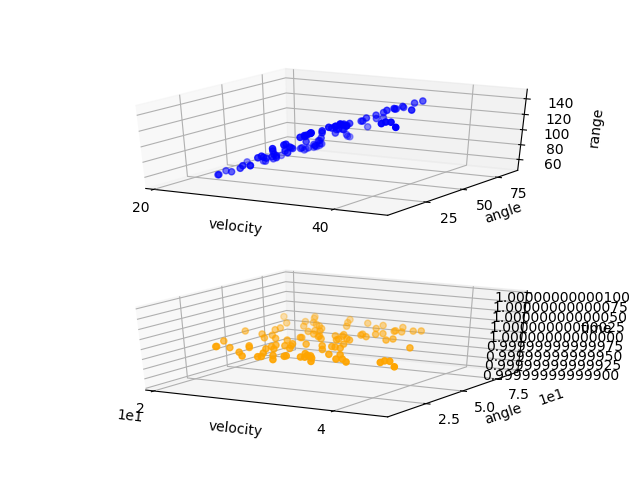
\includegraphics[scale=0.7]{../../tests/framework/user_guide/ForwardSamplingStrategies/gold/RunDir/SparseGrid/1-samplesROMPlot3D_scatter-scatter.png}
  \caption{Plot of validation samples generated by Monte Carlo sampling on the ROM.}
  \label{fig:samplesROMSparseGridPlot}
 \end{figure}
 %%%%%%%%%%%%%%%%%%%%%%%%%%%%%%%%%%%%%%%%%%%%%%%%%%%%%%%%%%









\input{adaptiveSamplingExample.tex}
\input{restartSampling.tex}
\section{Reduced Order Modeling through RAVEN}
\label{sec:ROMraven}
The development of high-fidelity codes, for thermal-hydraulic systems
and integrated multi-physics, has undergone a significant acceleration
in the last years. Multi-physics codes simulate
multiple physical models or multiple simultaneous physical phenomena,
in a integrated solving environment. Multi-physics typically
solves coupled systems of partial differential equations, generally
characterized by several different geometrical and time scales.

The new multi-physics codes are characterized by remarkable
improvements
in the approximation of physics (high approximation order and reduced
use of empirical correlations). This greater fidelity is generally
accompanied by a greater computational effort (increased calculation time). This peculiarity is an
obstacle in the application of  computational techniques of
quantification of uncertainty and risk associated with the operation of
particular industrial plant (e.g., a nuclear reactor).

A solution to this problem is represented by the
usage
of highly effective sampling strategies. Sometimes also these
approaches is not enough
in order to perform a comprehensive UQ and PRA analysis. In these
cases the help of reduced order modeling is essential.

RAVEN has support of several different ROMs,
such as:
\begin{enumerate}
  \item \textit{Nearest Neighbors approaches}
  \item \textit{Support Vector Machines}
  \item \textit{Inverse Weight regressors}
  \item \textit{Spline regressors }, etc.
\end{enumerate}

A ROM, also known a surrogate
model, is a mathematical representation of a system, used to predict
a FOM of a physical system.

The ``training'' is a process of setting the internal parameters of the ROM from a set
of samples generated the physical model, i.e.,
 the high-fidelity simulator (RELAP-7, RELAP5
3D, PHISICS, etc.),
\begin{figure}[h!]
  \centering
  \includegraphics[width=1.0\textwidth]  {pics/ROMexampleOfPhysicalSystem.png}
  \caption{Example of reduced order model representation of physical system (regression).}
  \label{fig:ROMexampleOfPhysicalSystem}
\end{figure}

Two characteristics of these models
are generally assumed (even if exceptions are possible):
\begin{enumerate}
  \item The higher the number of realizations in the training sets, the
higher is the accuracy of the prediction performed by the ROM is. This
statement is true for most of the cases, although some ROMs might be
subject to the over-fitting issues. The over-fitting phenomenon is not
analyzed here, since its occurrence highly depends on the
algorithm type, and, hence, the problem needs to be analyzed for all
the large number of ROM types available
  \item The smaller the size of the input (uncertain) domain with
  respect to the variability of the system response, the more likely the
  ROM is able to represent the system response space.
\end{enumerate}

The goals of this section are about learning how to:
 \begin{enumerate}
   \item Set up a sampling strategy to construct multiple ROMs, perturbing a driven code
   \item Train the different ROMs with the data-set obtained by the applied sampling strategy;
   \item Use the same sampling strategy, perturbing the ROMs
   \item Plot the responses of the driven code and ROMs, respectively.
\end{enumerate}
In order to accomplish these tasks, the following RAVEN \textbf{Entities} (XML blocks in the input files) need to be defined:
\begin{enumerate}
   \item \textbf{\textit{RunInfo}}:
     \xmlExample{framework/user_guide/ReducedOrderModeling/reducedOrderModeling.xml}{RunInfo}
   As in the other examples, the the \textit{RunInfo} \textbf{Entity} is intended  to set up the analysis sequence that
   needs to be performed. The number of steps specified in (\xmlNode{Sequence}) are sequentially run, eight steps in this specific case, using the number of processors assigned in (\xmlNode{batchSize}).
   \\In the first step, the model is going to be sampled. The obtained results are going to be used to  train three different ROMs.These ROMs are sampled by the same strategy used in the first step in order to compare the ROMs' responses with the ones coming from the original model.
   \item \textbf{\textit{Models}}:
     \xmlExample{framework/user_guide/ReducedOrderModeling/reducedOrderModeling.xml}{Models}
 As mentioned earlier, the goal of this example is the employment of
 a sampling strategy in order to construct multiple types of ROMs.
 \\Indeed, in addition to an External model,
 three different ROMs (GP, SVM and IDW) are here specified. The ROMs will be
 constructed (``trained'') through the data-set generated by the sampling of the External model. Once trained, they are going  to be used in place of the original model.
 \\As it can be seen, the ROMs will be constructed considering two features ($v0,\, and angle,\,$) and two targets  ($r \, and \, t$).
   \item \textbf{\textit{Distributions}}:
     \xmlExample{framework/user_guide/ReducedOrderModeling/reducedOrderModeling.xml}{Distributions}
  In the Distributions XML section, the stochastic model for the
  uncertainties are reported. In
  this case two distributions are defined:
  \begin{itemize}
    \item $vel\_dist \sim \mathbb{N}(30,5)$, used to model the uncertainties
    associated with  the \textit{velocity};
    \item  $angle\_dist \sim \mathbb{U}(5,85)$,  used to
    model the uncertainties associated with the \textit{angle}.
  \end{itemize}
   \item \textbf{\textit{Samplers}}:
     \xmlExample{framework/user_guide/ReducedOrderModeling/reducedOrderModeling.xml}{Samplers}
  To obtain the data-set on which the data mining algorithms are going to be applied, a \textit{MonteCarlo} sampling approach is employed here.
   \item \textbf{\textit{DataObjects}}:
     \xmlExample{framework/user_guide/ReducedOrderModeling/reducedOrderModeling.xml}{DataObjects}
  Int this block, six \textit{DataObjects} are defined: 1) PointSet
  named ``samples'' used to collect the final outcomes of the code, 2)
  HistorySet named ``histories'' in which the full time responses of the
  variables are going to be stored, 3) PointSet named
  ``inputPlaceHolder'' used in the \textit{role} of \xmlNode{Input} for the ROMs sampling;
  4) PointSet named ``samplesGP'' used to collect the final outcomes (sampling) of the Gaussian Process (GP) ROM;
  5) PointSet named ``samplesInverse'' used to collect the final outcomes (sampling) of the Inverse Distance Weighting (IDW) ROM;
  6) PointSet named ``samplesSVM'' used to collect the final outcomes (sampling) of the Support Vector Machine (SVM) ROM.
 %%%%%%%%%%%%%%%%%%%%%%%%%%%%%%%%%%%%%%%%%%%%%%%%%%%%%%%%%%
 %%%%%%%%%%%%%%%%%%%%%%%%%%%%%%%%%%%%%%%%%%%%%%%%%%%%%%%%%%
 %figure samples
 \begin{figure}[h!]
  \centering
  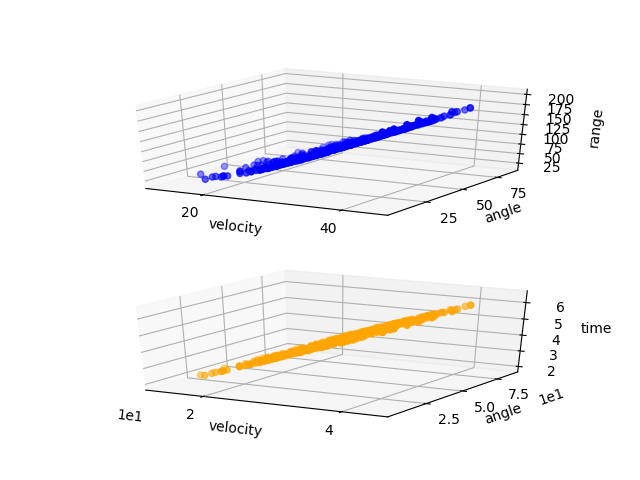
\includegraphics[scale=0.7]{../../tests/framework/user_guide/ReducedOrderModeling/gold/ROMConstruction/1-samplesPlot3D_scatter-scatter.png}
  \caption{Plot of the samples generated by the Monte Carlo sampling}
  \label{fig:ROMgrid_pointsets}
 \end{figure}
 %%%%%%%%%%%%%%%%%%%%%%%%%%%%%%%%%%%%%%%%%%%%%%%%%%%%%%%%%%
 %%%%%%%%%%%%%%%%%%%%%%%%%%%%%%%%%%%%%%%%%%%%%%%%%%%%%%%%%%
   \item \textbf{\textit{OutStreams}}:
     \xmlExample{framework/user_guide/ReducedOrderModeling/reducedOrderModeling.xml}{OutStreams}
     This model makes use of two Print OutStreams and five Plot OutStreams:
     \begin{itemize}
       \item ``samples,'' which writes the contents of the point-wise training samples to CSV,
       \item ``histories,'' which writes the contents of the history-wise training samples to linked CSVs,
       \item ``historyPlot,'' which plots the evolution of the training samples,
       \item ``samplesPlot3D,'' which plots the final state of the training samples with relation to the
         outputs of interest,
       \item ``samplesPlot3DROMgp,'' which plots the validation samples of the Gaussian Process ROM,
       \item ``samplesPlot3DROMsvm,'' which plots the validation samples of the Support-Vector Machine ROM,
       \item ``samplesPlot3Dinverse,'' which plots the validation samples of the multidimensional Inverse
         Weight ROM.
     \end{itemize}
     The 3D plots of the samples as well as the ROM samples can be used as a view-norm validation of the ROMs.
   \item \textbf{\textit{Steps}}:
     \xmlExample{framework/user_guide/ReducedOrderModeling/reducedOrderModeling.xml}{Steps}
  %%%%%%%%%%%%%%%%%%%%%%%%%%%%%%%%%%%%%%%%%%%%%%%%%%%%%%%%%%
 %figure samples
 \begin{figure}[h!]
  \centering
  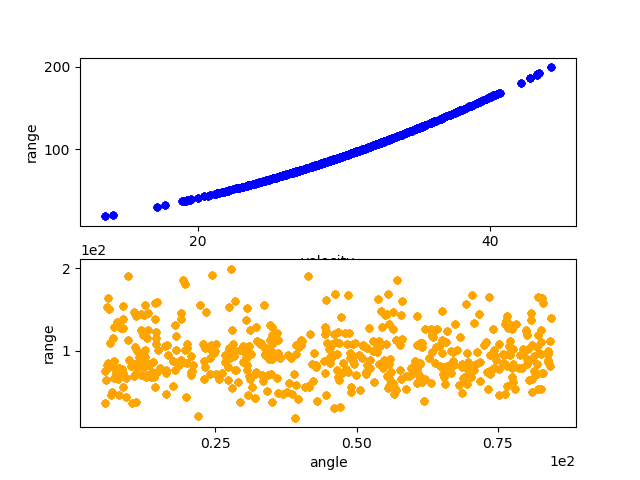
\includegraphics[scale=0.7]{../../tests/framework/user_guide/ReducedOrderModeling/gold/ROMConstruction/1-historyPlot_scatter-scatter.png}
  \caption{Plot of the histories generated by the Monte Carlo method}
  \label{fig:ROMgrid_histories}
 \end{figure}
   %%%%%%%%%%%%%%%%%%%%%%%%%%%%%%%%%%%%%%%%%%%%%%%%%%%%%%%%%%
 %figure samples
 \begin{figure}[h!]
  \centering
  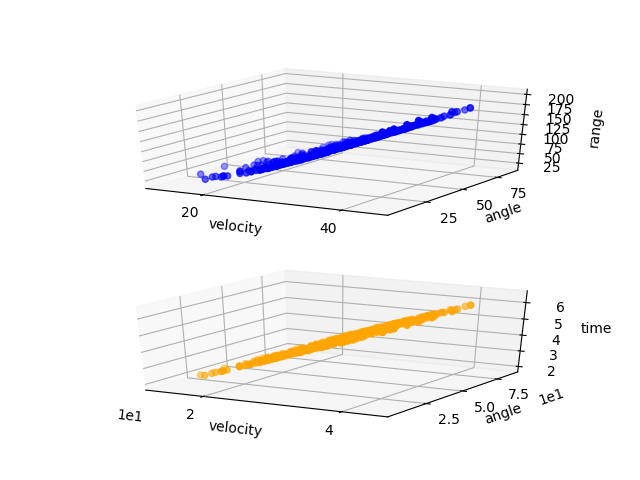
\includegraphics[scale=0.7]{../../tests/framework/user_guide/ReducedOrderModeling/gold/ROMConstruction/1-samplesPlot3DROMgp_scatter-scatter.png}
  \caption{Plot of the samples generated by the Monte Carlo sampling applied on the Gaussian Process ROM}
  \label{fig:ROMgp_samples}
 \end{figure}
 %%%%%%%%%%%%%%%%%%%%%%%%%%%%%%%%%%%%%%%%%%%%%%%%%%%%%%%%%%
 %%%%%%%%%%%%%%%%%%%%%%%%%%%%%%%%%%%%%%%%%%%%%%%%%%%%%%%%%%
   Finally, all the previously defined \textbf{Entities} can be combined in
   the \xmlNode{Steps} block. As inferable,
   eight \xmlNode{Steps} have been inputted:
   \begin{itemize}
     \item \xmlNode{MultiRun} named ``sample'', used to run the multiple
     instances of the driven code and
     collect the outputs in the two \textit{DataObjects}. As it can be
     seen, the \xmlNode{Sampler} is inputted to communicate to the
     \textit{Step} that the driven code needs to
     be perturbed through the Grid sampling strategy;
     \item \xmlNode{RomTrainer} named ``trainROMGaussianProcess'', used to construct (``train'')
     the GP ROM, based on the data-set generated in the  ``sample'' \textbf{Step};
     \item \xmlNode{RomTrainer} named ``trainROMsvm'', used to construct (``train'')
     the SVM ROM, based on the data-set generated in the  ``sample'' \textbf{Step};
     \item \xmlNode{RomTrainer} named ``trainROMinverse'', used to construct (``train'')
     the IDW ROM, based on the data-set generated in the  ``sample'' \textbf{Step};
     \item \xmlNode{MultiRun} named ``sampleROMGaussianProcess'', used to run the multiple
     instances of the previously constructed GP ROM and
     collect the outputs in the PointSet \textit{DataObject}. As it can be
     seen, the same \xmlNode{Sampler} used for perturbing the original model is here used.
     \item \xmlNode{MultiRun} named ``sampleROMsvm'', used to run the multiple
     instances of the previously constructed Support Vector Machine ROM and
     collect the outputs in the PointSet \textit{DataObject}. As it can be
     seen, the same \xmlNode{Sampler} used for perturbing the original model is here used.
     \item \xmlNode{MultiRun} named ``sampleROMInverse'', used to run the multiple
     instances of the previously constructed Inverse Distance Weight ROM and
     collect the outputs in the PointSet \textit{DataObject}. As it can be
     seen, the same \xmlNode{Sampler} used for perturbing the original model is here used.
     \item  \xmlNode{IOStep} named ``writeHistories'', used to 1) export
     the ``histories'' and ``samples''  \textit{DataObjects}
     \textbf{Entity} in a CSV file and 2) plot the responses of the sampling performed on the physical model, GP ROM,
     SVM ROM and IDW ROM in  PNG files and on the screen.
   \end{itemize}
\end{enumerate}

  %figure samples
 \begin{figure}[h!]
  \centering
  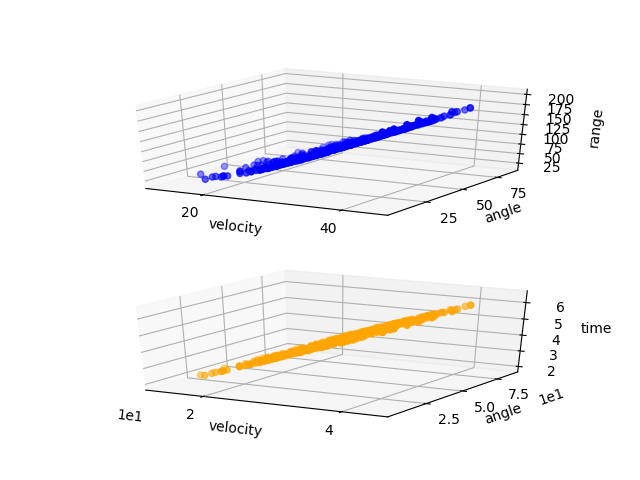
\includegraphics[scale=0.7]{../../tests/framework/user_guide/ReducedOrderModeling/gold/ROMConstruction/1-samplesPlot3DROMsvm_scatter-scatter.png}
  \caption{Plot of the samples generated by the Monte Carlo sampling applied on the Support Vector Machine ROM}
  \label{fig:ROMsvm_samples}
 \end{figure}
 %%%%%%%%%%%%%%%%%%%%%%%%%%%%%%%%%%%%%%%%%%%%%%%%%%%%%%%%%%
  %%%%%%%%%%%%%%%%%%%%%%%%%%%%%%%%%%%%%%%%%%%%%%%%%%%%%%%%%%
  %figure samples
 \begin{figure}[h!]
  \centering
  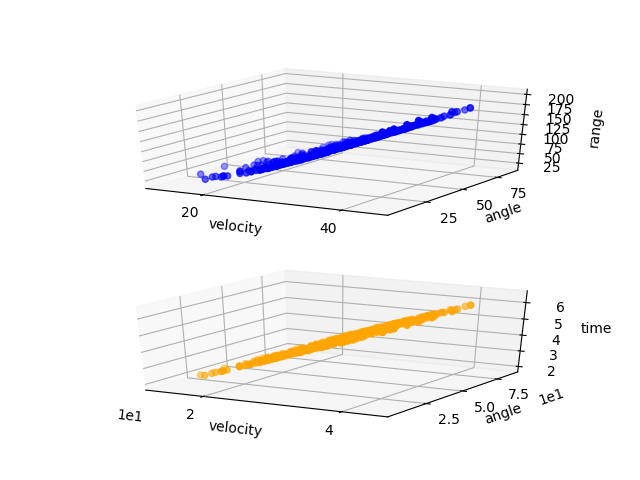
\includegraphics[scale=0.7]{../../tests/framework/user_guide/ReducedOrderModeling/gold/ROMConstruction/1-samplesPlot3DROMinverse_scatter-scatter.png}
  \caption{Plot of the samples generated by the Monte Carlo sampling applied on the Inverse Distance Weight ROM}
  \label{fig:ROMinverse_samples}
 \end{figure}
 %%%%%%%%%%%%%%%%%%%%%%%%%%%%%%%%%%%%%%%%%%%%%%%%%%%%%%%%%%
 Figure \ref{fig:ROMgrid_histories}
 shows the range $r$ for different velocity and angle.
 Figure \ref{fig:ROMgrid_pointsets} shows the final responses  of the sampling employed using the driven code.

Figures \ref{fig:ROMgp_samples}, \ref{fig:ROMsvm_samples} and \ref{fig:ROMinverse_samples}  show the final responses  of the sampling employed using the Gaussian Process, Support Vector Machines and Inverse Distance Weight ROMs, respectively.
It can be clearly noticed that the responses of the ROMs perfectly match the outcomes coming from the original model (see Figure   \ref{fig:ROMgrid_pointsets}).









\section{Statistical Analysis through RAVEN}
\label{sec:SAraven}
In order to perform a complete analysis of a system under uncertainties,
it is crucial to be able to compute all the statistical moments of one or even multiple
FOMs. In addition, it is essential to identify the correlation
among different FOMs toward a specific input space.

RAVEN is able to compute the most important statistical moments:
such as:
\begin{enumerate}
  \item \textit{Expected Value}
  \item \textit{Standard Deviation}
  \item \textit{Variance}
  \item \textit{variationCoefficient}
  \item \textit{Skewness}
  \item \textit{Kurtosis}
  \item \textit{Median}
  \item \textit{Percentile}.
\end{enumerate}
In addition, RAVEN fully supports the computation of all of the statistical moments defined to
``measure'' the correlation among variables/parameters/FOMs:
\begin{enumerate}
  \item \textit{Covariance matrix}
  \item \textit{Normalized Sensitivity matrix}
  \item \textit{Variance Dependent Sensitivity matrix}
  \item \textit{Sensitivity matrix}
  \item \textit{Pearson matrix}.
\end{enumerate}
The goals of this section is to show how to:
 \begin{enumerate}
   \item Set up a sampling strategy to perform a final statistical analysis
   perturbing a driven code
   \item Compute all the statistical moments and correlation/covariance
   metrics.
\end{enumerate}
In order to accomplish these tasks, the following RAVEN \textbf{Entities} (XML blocks in the input files) need to be defined:
\begin{enumerate}
   \item \textbf{\textit{RunInfo}}:
     \xmlExample{framework/user_guide/StatisticalAnalysis/statisticalAnalysis.xml}{RunInfo}
   As shown in the other examples, the \textit{RunInfo} \textbf{Entity} is intended  to set up the desired analysis. The number of steps specified in (\xmlNode{Sequence}) are sequentially run, two steps in this specific case, using the number of processors assigned in (\xmlNode{batchSize}).
   \\In the first step, the original physical model is sampled. The obtained results are  analyzed with the Statistical Post-Processor.
   \item \textbf{\textit{Models}}:
     \xmlExample{framework/user_guide/StatisticalAnalysis/statisticalAnalysis.xml}{Models}
 The goal of this example is to show how the
 principal statistical FOMs can be computed through RAVEN.
 \\We use an External model and specify a Post-Processor model (BasicStatistics). The post-process step is performed on all the output FOMs used in this example ($r and t$).
   \item \textbf{\textit{Distributions}}:
     \xmlExample{framework/user_guide/StatisticalAnalysis/statisticalAnalysis.xml}{Distributions}
  In the Distributions XML section, the stochastic model for the
  uncertainties are reported. In this case 2 distributions are defined:
  \begin{itemize}
    \item $vel\_dist \sim \mathbb{N}(30,5)$, used to model the uncertainties
    associated with  the \textit{velocity};
    \item  $angle\_dist \sim \mathbb{U}(5,85)$,  used to
    model the uncertainties associated with the \textit{angle}.
  \end{itemize}
   \item \textbf{\textit{Samplers}}:
     \xmlExample{framework/user_guide/StatisticalAnalysis/statisticalAnalysis.xml}{Samplers}
  In order to obtain the data-set on which the data mining algorithms are going to be applied, a \textit{MonteCarlo} sampling approach is employed here.
   \item \textbf{\textit{DataObjects}}:
     \xmlExample{framework/user_guide/StatisticalAnalysis/statisticalAnalysis.xml}{DataObjects}
  In this block, three \textit{DataObjects} are defined:
  1) PointSet named ``samples'' used to collect the final outcomes of
  the code,
  2) PointSet named ``dummyIN'' used as a placeholder for the \textit{Multirun} step,
  3) HistorySet named ``histories'' in which the full time responses of the
  variables $x,y,t$ are going to be stored.

   \item \textbf{\textit{Steps}}:
     \xmlExample{framework/user_guide/StatisticalAnalysis/statisticalAnalysis.xml}{Steps}

 %%%%%%%%%%%%%%%%%%%%%%%%%%%%%%%%%%%%%%%%%%%%%%%%%%%%%%%%%%
 %%%%%%%%%%%%%%%%%%%%%%%%%%%%%%%%%%%%%%%%%%%%%%%%%%%%%%%%%%
   Finally, all the previously defined \textbf{Entities} can be combined in
   the \xmlNode{Steps} block. As inferable,
   2 \xmlNode{Steps} have been inputted:
   \begin{itemize}
     \item \xmlNode{MultiRun} named ``sampleMC'', used to run the
     multiple
     instances of the driven code and
     collect the outputs in the two \textit{DataObjects}. As it can be
     seen, the \xmlNode{Sampler} is inputted to communicate to the
     \textit{Step} that the driven code needs to
     be perturbed through the MonteCarlo sampling strategy.
     \item \xmlNode{PostProcess} named ``statisticalAnalysisMC'', used
     compute all the statistical moments and FOMs based on the
     data obtained through the sampling strategy. As it can be noticed,
     the \xmlNode{Output} of the ``sampleMC'' \textit{Step} is the
     \xmlNode{Input} of the ``statisticalAnalysisMC''  \textit{Step}.
   \end{itemize}
\end{enumerate}

Tables \ref{ScalarMoments}-\ref{SensitivityComputed} show all the results of the \textit{PostProcess}
step.


\begin{table}[h!]
\centering
\caption{Computed Moments and Cumulants}
\label{ScalarMoments}
\begin{tabular}{|c|c|c|}
\hline
{\ul \textit{\textbf{Computed Quantities}}} & \textbf{r} & \textbf{t} \\ \hline
\textit{expected value}                     & 65.88   & 3.94   \\ \hline
\textit{median}                             & 61.74   & 4.12   \\ \hline
\textit{variance}                           & 1022.01 & 3.53   \\ \hline
\textit{sigma}                              & 31.97   & 1.89  \\ \hline
\textit{variation coefficient}              & 0.48    & 0.48   \\ \hline
\textit{skewness}                           & 0.55    & -0.03  \\ \hline
\textit{kurtosis}                           & -0.01   & -0.96  \\ \hline
\textit{percentile 5\%}                     & 20.21   & 0.85   \\ \hline
\textit{percentile 95\%}                    & 122.83  & 6.90   \\ \hline
\end{tabular}
\end{table}
\begin{table}[h!]
\centering
\caption{Covariance matrix.}
\label{covarianceComputed}
\begin{tabular}{|c|c|c|}
\hline
{\ul \textit{\textbf{Covariance}}} & \textbf{r} & \textbf{t} \\ \hline
\textit{velocity}                     & 95.36   & 3.29   \\ \hline
\textit{angle}                        & 25.29   & 40.42   \\ \hline
\end{tabular}
\end{table}
\begin{table}[h!]
\centering
\caption{Correlation matrix}
\label{pearsonComputed}
\begin{tabular}{|c|c|c|}
\hline
{\ul \textit{\textbf{Correlation}}} & \textbf{r} & \textbf{t} \\ \hline
\textit{velocity}                     & 0.61   & 0.36   \\ \hline
\textit{angle}                        & 0.03   & 0.92   \\ \hline
\end{tabular}
\end{table}
\begin{table}[h!]
\centering
\caption{Variance Dependent Sensitivity matrix}
\label{VarDepSensitivityComputed}
\begin{tabular}{|c|c|c|}
\hline
{\ul \textit{\textbf{Variance Sensitivity}}} & \textbf{r} & \textbf{t} \\ \hline
\textit{velocity}                     & -1.69   & 0.08   \\ \hline
\textit{angle}                        & -3.31   & 0.07   \\ \hline
\end{tabular}
\end{table}
\begin{table}[h!]
\centering
\caption{Sensitivity matrix}
\label{SensitivityComputed}
\begin{tabular}{|c|c|c|}
\hline
{\ul \textit{\textbf{Sensitivity (I/O)}}} & \textbf{r} & \textbf{t} \\ \hline
\textit{velocity}                     & 3.95   & 0.12   \\ \hline
\textit{angle}                        & 0.01   & 0.07   \\ \hline
\end{tabular}
\end{table}


\section{Data Mining through RAVEN}
\label{sec:DMraven}

Data mining is the computational process of discovering patterns in large data sets (``big data'') involving methods at the intersection of artificial intelligence, machine learning, statistics, and database systems. The overall goal of the data mining process is to extract information from a data set and transform it into an understandable structure for further use.
\\RAVEN has support of several different data mining algorithms,
such as:
\begin{enumerate}
  \item \textit{Hierarchical methodologies}
  \item \textit{K-Means}
  \item \textit{Mean-Shift}, etc.
\end{enumerate}

The goals of this section are about learning how to:
 \begin{enumerate}
   \item Set up a sampling strategy to apply clustering algorithms, perturbing a driven code
  \item Analyze the data using clustering algorithms.
\end{enumerate}
To accomplish these tasks, the following RAVEN \textbf{Entities} (XML blocks in the input files) need to be defined:
\begin{enumerate}
   \item \textbf{\textit{RunInfo}}:
     \xmlExample{framework/user_guide/DataMining/dataMiningAnalysis.xml}{RunInfo}
   The \textit{RunInfo} \textbf{Entity} is intended  to set up the analysis sequence that
   needs to be performed. The number of steps specified in (\xmlNode{Sequence}) are sequentially run
   using the number of processors assigned in (\xmlNode{batchSize}).
   \\In the first step, the original physical model is going to be sampled.
   The obtained results are going to be analyzed with data mining
   algorithms.
   \item \textbf{\textit{Models}}:
     \xmlExample{framework/user_guide/DataMining/dataMiningAnalysis.xml}{Models}
 The goal of this example is to show how the
 data mining algorithms in RAVEN can be useful to analyze large data set.
 \\In addition to an External model, two Post-Processor models ($DataMining|cluster|KMeans$ and $DataMining|decomposition|PCA$) are specified. Note that the post-processing is performed on all the output FOMs used in this example ($r and t$).
   \item \textbf{\textit{Distributions}}:
     \xmlExample{framework/user_guide/DataMining/dataMiningAnalysis.xml}{Distributions}
  In the Distributions XML section, the stochastic model for the
  uncertainties are reported. In this case 2 distributions are defined:
  \begin{itemize}
    \item $vel\_dist \sim \mathbb{N}(30,5)$, used to model the uncertainties
    associated with  the \textit{velocity};
    \item  $angle\_dist \sim \mathbb{U}(5,85)$,  used to
    model the uncertainties associated with the \textit{angle}.
  \end{itemize}
   \item \textbf{\textit{Samplers}}:
     \xmlExample{framework/user_guide/DataMining/dataMiningAnalysis.xml}{Samplers}
  In order to obtain the data-set on which the data mining algorithms are going to be applied, a \textit{MonteCarlo} sampling approach is employed here.
   \item \textbf{\textit{DataObjects}}:
     \xmlExample{framework/user_guide/DataMining/dataMiningAnalysis.xml}{DataObjects}
  In this block, three \textit{DataObjects} are defined:
  1) PointSet named ``samples'' used to collect the final outcomes of
  the code,
  2) PointSet named ``dummyIN'' used as a placeholder for the \textit{Multirun} step,
  3) HistorySet named ``histories'' in which the full time responses of the
  variables $x,y,t$ are going to be stored.
 %figure samples
 \begin{figure}[h!]
  \centering
  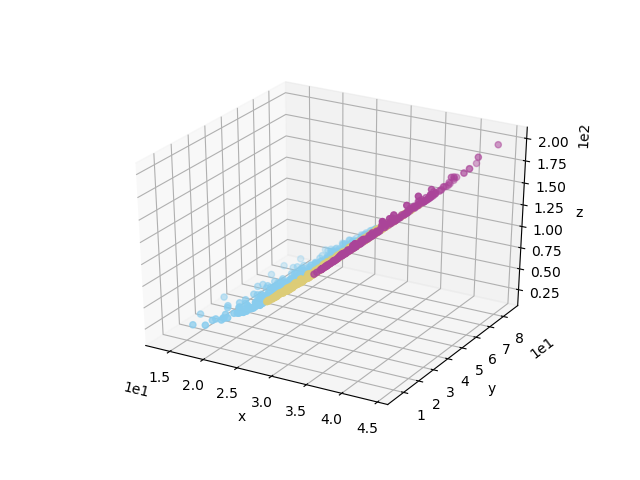
\includegraphics[scale=0.7]{../../tests/framework/user_guide/DataMining/gold/dataMiningAnalysis/1-PlotLabels_dataMining.png}
  \caption{K-means clustering on original dataset.}
  \label{fig:KmeanOrigData}
 \end{figure}
   \item \textbf{\textit{OutStreams}}:
     \xmlExample{framework/user_guide/DataMining/dataMiningAnalysis.xml}{OutStreams}
     This workflow uses one Print OutStream and three Plot OutStreams:
     \begin{itemize}
       \item ``samplesDump'', which writes the original sample set with the additional columns from the
         PostProcess steps,
       \item ``PlotKMeans1'', which plots the samples against the Figures of Merit with coloring according to the KMeans clustering,
       \item ``PlotLabels'', which plots the samples and colors them according to the KMeans clustering,
       \item ``PlotPCA1,'' which plots the surrogate principal component dimensions and their associated clustering.
     \end{itemize}
     Note that a special kind of plot, the ``dataMining'' \xmlNode{type}, has been implemented to simplify plotting complicated results using RAVEN, and is used in all three of the plots in this workflow.  Also note the use of the \xmlNode{range} block to define the data range of the plots created.
   \item \textbf{\textit{Steps}}:
     \xmlExample{framework/user_guide/DataMining/dataMiningAnalysis.xml}{Steps}

 %%%%%%%%%%%%%%%%%%%%%%%%%%%%%%%%%%%%%%%%%%%%%%%%%%%%%%%%%%
 %%%%%%%%%%%%%%%%%%%%%%%%%%%%%%%%%%%%%%%%%%%%%%%%%%%%%%%%%%
   Finally, all the previously defined \textbf{Entities} can be combined in
   the \xmlNode{Steps} block;
   3 \xmlNode{Steps} have been inputted:
   \begin{itemize}
     \item \xmlNode{MultiRun} named ``sample'', used to run the
     multiple
     instances of the driven code and
     collect the outputs in the two \textit{DataObjects}.The \xmlNode{Sampler} is inputted to communicate to the
     \textit{Step} that the driven code needs to
     be perturbed through the MonteCarlo sampling strategy;
     \item \xmlNode{PostProcess} named ``kmeans'', used
     to analyze the data obtained through the sampling strategy. In
     this step, a K-Means algorithm is going to be employed, plotting
     the clustering results;
     \textit{Step} that the driven code needs to
     be perturbed through the MonteCarlo sampling strategy;
     \item \xmlNode{PostProcess} named ``pca'', used
     to analyze the data obtained through the sampling strategy. In
     this Step, a PCA algorithm is going to be employed, plotting
     the decomposition results.
   \end{itemize}
\end{enumerate}
Figure~\ref{fig:KmeanOrigData} shows the clustering on the input space and the range, coloring according to the KMeans clustering,.
\\Figure~\ref{fig:KmeanProjected} shows the clustering on the range-angle and range-velocity plots respectively.
\\Figure~\ref{fig:PCAplot} shows the PCA decomposition on the data set.
%%%%%%%%%%%%%%%%%%%%%%%%%%%%%%%%%%%%%%%%%%%%%%%%%%%%%%%%%%
 %figure samples
 \begin{figure}[h!]
  \centering
  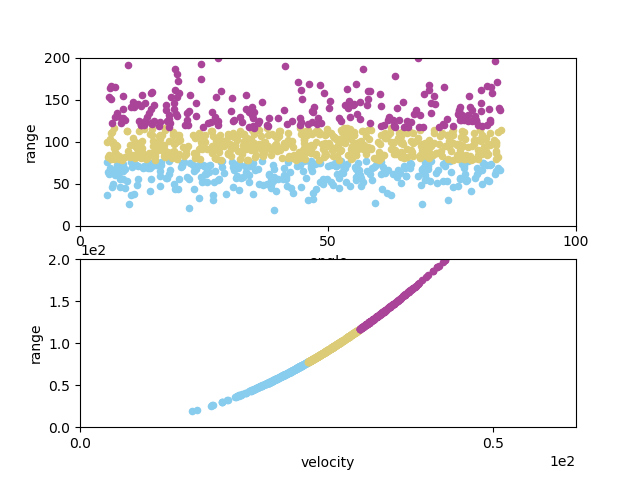
\includegraphics[scale=0.7]{../../tests/framework/user_guide/DataMining/gold/dataMiningAnalysis/1-PlotKMeans1_dataMining-dataMining.png}
  \caption{K-means clustering on projected parameters.}
  \label{fig:KmeanProjected}
 \end{figure}
 %%%%%%%%%%%%%%%%%%%%%%%%
 %%%%%%%%%%%%%%%%%%%%%%%%%%%%%%%%%%%%%%%%%%%%%%%%%%%%%%%%%%

 %%%%%%%%%%%%%%%%%%%%%%%%
  %%%%%%%%%%%%%%%%%%%%%%%%%%%%%%%%%%%%%%%%%%%%%%%%%%%%%%%%%%
 %figure samples
 \begin{figure}[h!]
  \centering
  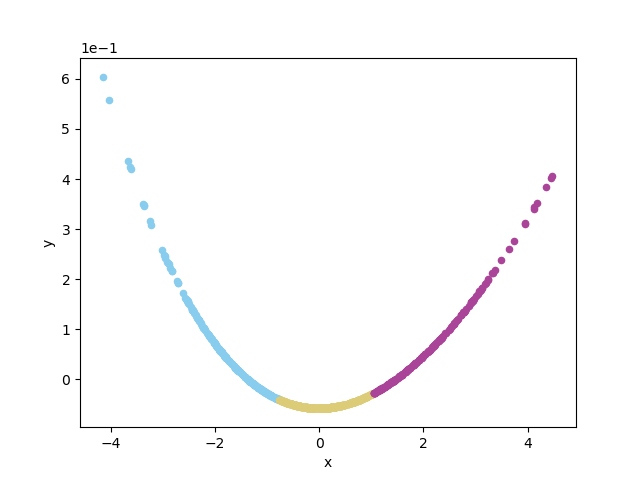
\includegraphics[scale=0.7]{../../tests/framework/user_guide/DataMining/gold/dataMiningAnalysis/1-PlotPCA1_dataMining.png}
  \caption{Principal Component Analysis.}
  \label{fig:PCAplot}
 \end{figure}
 %%%%%%%%%%%%%%%%%%%%%%%%


\section{Model Optimization}
\label{sec:optimizerStrategies}

When analyzing the range of values obtainable by a model, frequently a key question is ``what set of
parameters result in the best response value?''  To answer this question, RAVEN uses the \xmlNode{Optimizer},
a powerful sampler-like entity that searches the input space to find minimum or maximum values of a response.

In the remainder of this section, we will explore how to use the optimizer using a simple analytic problem,
with a two-dimensional input space and single response of interest.  After getting used to running with the
optimizer, we will add increasing complexity, including changing adaptive step sizes, initial conditions,
parallel trajectories, input space subdivision, input space constraints, and response constraints.

To demonstrate the operation of the Optimizer entities in RAVEN, the model we consider is the Beale function,
which is documented in the analytic tests for RAVEN and replicated here:

\begin{itemize}
  \item Function: $f(x,y) = (1.5-x+xy)^2+(2.25-x+xy^2)^2+(2.625-x+xy^3)^2$
  \item Domain: $-4.5 \leq x,y \leq 4.5$
  \item Global Minimum: $f(3,0.5)=0$
\end{itemize}

The two inputs are the variables $x$ and $y$, and the response is a value we'll assign to $ans$, short for
``answer''.  The model is an external model in RAVEN, and can be found at
\begin{verbatim}
  raven/tests/framework/AnalyticModes/optimizing/beale.py.
\end{verbatim}
The function's values are distributed as in Fig. \ref{fig:beale}, with red indicating high values
and blue indicating low values.
\begin{figure}[h!]
  \centering
  \includegraphics[scale=0.7]{../../tests/framework/user_guide/optimizing/Beale_grid.png}
  \caption{Plot of Beale's function for Optimization}
  \label{fig:beale}
\end{figure}
The objective is to minimize the function.

Note that throughout this example we use the SPSA optimizer by way of demonstration, since it is the first
advanced algorithm for optimization included in RAVEN; many of the options and parameters apply to other
optimizers, and details can be found in the RAVEN user manual.

\subsection{Introduction: The Optimizer Input}
As with other entities, the Optimizer gets its own XML block in the RAVEN input.
Here's an example of an input for a SPSA optimizer named \xmlString{opter}:
\xmlExample{framework/user_guide/optimizing/simple.xml}{Optimizers}
This is the smallest amount of input needed to run an optimization problem, with the exception that we include
the \xmlNode{initialSeed} to maintain consistent results.  Note the required blocks included
to define the optimizer:
\begin{itemize}
  \item \xmlNode{objective}, which is where you indicate the variable for which you want to find the minimum (or,
    if you change the default, maximum).  As listed here, we want to minimize the value of \texttt{ans} given a
    range of possible values for \texttt{x} and \texttt{y}.
  \item \xmlNode{variable}, which is where you can define the input space variables, one for each of these
    nodes.  Declaring a variable here informs the optimizer that you want it to find the optimal value for
    this variable, along with the other variables declared in their own blocks. Note this follows
    the same pattern as any other \xmlNode{Sampler}, including a \xmlNode{distribution} node to
    describe the domain of the variable. For \xmlNode{GradientDescent}, the shape of the
    distribution is not significant unless performing other advanced optimizations (such as
    optimization at risk). Nominally, this distribution simply defines the acceptable range of the
    variable, making the \xmlNode{Uniform} distribution a common choice. The distribution sets the
    upper and lower bounds of the variable, which will give the optimizer some general expectations for
    finding the optimal point; it will never try to sample a value smaller than the lower bound or larger than
    the upper bound.  In the example we define variables \emph{x} and \emph{y} as our input variables, and
    both of them coincidentally range between -4.5 and 4.5.  We set the initial values for both variables to 0
    through the \xmlNode{initial} block, which is required in most cases; the exception is when a
    preconditioner sets them in mulitlevel optimization, but we're not concerned with that feature
    for this example.
  \item \xmlNode{TargetEvaluation}, which declares the DataObject that the optimization search evaluations are
    going to be placed in.  All of the optimal points found as part of the optimization, as well as any other
    points evaluated as part of the algorithm, are placed in this object so the optimizer can retrieve this
    information later.  When this data object is defined, it is critical that the objective variable is
    defined in the output space, and the input variables in the input space, so the optimizer can collect the
    results of its sampling.  The data object type should be ``PointSet'' for this data object.  In this
    example, we use the self-descriptive \emph{optOut} data object.
  \item \xmlNode{samplerInit}, which contains initialization parameters for the optimization
    algorithm. In this case, we set an \xmlNode{initialSeed} to 1234 just to maintain consistent
    results. We also set the maximum number of model evaluations through the \xmlNode{limit} node.
    We don't expect to need all these runs, but in case the optimizer is struggling, we set this
    cutoff to prevent the code running ad infinitum.
  \item \xmlNode{gradient}, which defines the gradient approximation algorithm to use within the
    gradient descent algorithm. In this case,
    we simply indicate that we want to use \xmlNode{SPSA}, and need no additional inputs.
  \item \xmlNode{stepSize}, which defines how we should control the step size during the gradient
    descent algorithm. There are several algorithms to choose from; in this case, we choose
    \xmlNode{GradientHistory}, which uses the scalar product between successive steps to determine
    what step to take in the search algorithm. A bigger growth factor results in traversing the input space more
    quickly, but converging more slowly. A bigger shrink factor results in collapsing to a minimum
    more quickly, converging quickly but possibly falling into local minima. We're using the default
    growth (1.25) and shrink (1.15) factors here.
  \item \xmlNode{acceptance}, which determines the algorithm by which we decide whether to accept a
    potential new optimal point during the gradient descent algorithm. In this case we use
    \xmlNode{Strict}, which indicates any potential new optimal points in the search that are not
    preferrable to the previously-found optimal point are discarded, and the search continues from
    the previously-found optimal point in the search.
  \item \xmlNode{convergence}, which informs the searching algorithm of when to decide it has found
    the optimal point within a sufficient tolerance. There are several stopping criteria; in this
    case, we use the local value of the \xmlNode{gradient}, which we want to be at most 0.1.
\end{itemize}
The other critical blocks in this input are as follows:

\subsubsection{Models}
\xmlExample{framework/user_guide/optimizing/simple.xml}{Models}
Note that we define the external model with the name \xmlString{beale} and provide a path to the analytic
model itself.  This model is set up with the \texttt{run} method that allows RAVEN to run the model.  We also
list all our input/output variables, \emph{x, y}, and \emph{ans}.

\subsubsection{Data Objects}
\xmlExample{framework/user_guide/optimizing/simple.xml}{DataObjects}
We have three data objects:
\begin{itemize}
\item \xmlString{placeholder}, which is necessary to define the input to our external
model in the Steps (the external model doesn't use any input file, so we just use a placeholder
here);
\item \xmlString{optOut}, which will hold all of the samples taken by our optimizer (optimal
candidates, gradient evaluation points, rejected points, etc); and
\item \xmlString{opt\_export}, which will hold the actual solution path taken by our optimizer.  We store the
path travelled by the optimization algorithm as successive samples, with \texttt{iteration} keeping track of the
optimization steps taken.  Note especially how the input of \xmlString{opt\_export} is set to \texttt{trajID},
which is a special keyword for the Optimizer trajectory tracking, as is the output variable \texttt{iteration}.
There are several other special keyword outputs that can be written to the Solution Export data object, that
can be found in the user manual.
\end{itemize}

\subsubsection{Out Streams}
\xmlExample{framework/user_guide/optimizing/simple.xml}{OutStreams}
Here we define the way to print the output of our optimization algorithm.  There's not much to note, except
that we'll be printing the optimization path as a CSV.

\subsubsection{Steps}
\xmlExample{framework/user_guide/optimizing/simple.xml}{Steps}
Here we put it all together into a work flow that RAVEN can follow.  We only need two steps: one to optimize,
and one to print out the results.  To actually perform the optimization, we need a MultiRun step, which we
cleverly name \xmlString{optimize}.  For input we take the placeholder data object \emph{placeholder}, which sets
up the input space of the model we defined, \emph{beal}.  Where a \xmlNode{Sampler} would normally go, we
include the \xmlNode{Optimizer} we defined earlier.  We output to the same data object we indicated in the
Optimizer's \xmlNode{TargetEvaluation} node.  Finally, we note specifically the use of the
\xmlNode{SolutionExport} node.  The data object defined in this node is where the Optimizer will write the
optimization path history, with the final entry being the last step taken by the optimizer.  The IOStep is
unremarkable, used simply to write out the optimization path history to file.

\subsubsection{Conclusion}
After reviewing the components (don't forget the RunInfo block!), you can run this example and see the
results.  In particular, we can view the final results of the optimizer in \texttt{Simple/opt\_export\_0.csv}.  Note
that \texttt{opt\_export} is the name of the \xmlNode{Print} OutStream we defined in the input file.

When we open the file (preferably in a CSV reader such a spreadsheet viewer), we see a CSV with several headers,
the outputs defined in the data object in the input
file: \emph{trajID}, \emph{iteration}, \emph{x}, \emph{y}, and \emph{ans} (not necessarily in that order).  \emph{x},
\emph{y}, and \emph{ans} are the values of the variable at each optimization iteration, while
\emph{iteration} gives the sequential order of the optimization iteration. \emph{trajID} is the
trajectory identifying number; since we are only using one trajectory, this identifier is simply 0.

We can see there's only one line of data in the ouput CSV, showing the final solution discovered by
the optimization algorithm.
If we look at the line, we converged around $f(2.7, 0.42) = 0.0199$ in 40 steps, which is okay but still a little
ways from the analytic optimal point $f(3, 0.5) = 0$.  If we look at the output from the run, we can look at
the last time RAVEN was ``Checking convergence for Trajectory 0''.  Below that statement, there are a series
of convergence criteria and their respeective statuses.  We can see our convergence criteria
requested through the input file (\texttt{gradient}, whose final accepted value is 0.0857) as well
as the \texttt{same point} convergence criteria, which helps determine if the optimal solution is at
a boundary even though other conditions have not converged.

We can see that the reason we converged at the end is the
\texttt{gradient}, which means the relative change in the gradient of \emph{ans} was sufficiently
small between steps to cause convergence.  Clearly, we claimed convergence prematurely because of
the low value required in the optimizer input.  Because these convergence criteria are very
problem-specific, one set parameters will not work best for all problems.

We can improve this result by changing convergence
parameters as well as step size growth and shrink factors, all of which can be found in the user manual, and
many of which we'll discuss in the rest of this section. Feel free to experiment with these values,
and see their affect on the solution discovered.

\subsection{Increasing verbosity}
We saw in the previous section that the output stored in \texttt{Simple/opt\_export.csv} only
includes the final optimal solution, and minimal information about that point. We can increase the
output to see the entire path traversed by adding a few parameters in the input file.

The first parameter to add is in \xmlNode{Optimizers} \xmlNode{GradientDescent}
\xmlNode{samplerInit}. By adding the node \xmlNode{writeSteps} with the value \xmlString{every}, we
can see the full path taken by the optimizer from initial point to final accepted solution.

Further, the optimizer has some special variables that can be use in the \xmlNode{SolutionExport}
\xmlNode{DataObject} to print additional information to the CSV. For example, the special variable
\texttt{accepted} will tell us, for each point in the optimization path, what the result of that
point is. For SPSA, these acceptance notes can be one of the following:
\begin{itemize}
  \item \texttt{first}, or the initial point at which the optimization search begins;
  \item \texttt{accepted}, if the new proposed point is sufficiently improved to be accepted as a
    new optimal point in the search;
  \item \texttt{rejected}, if the new proposed point is \emph{not} sufficiently improved and
    therefore rejected;
  \item \texttt{rerun}, indicating the search algorithm returned to an old optimal point after
    rejecting a proposed optimal point; and
  \item \texttt{final}, which shows that the point listed is the final accepted and converged
    optimal point.
\end{itemize}



\subsection{Initial Conditions and Parallel Trajectories} \label{subsec:opt parallel traj}
Notice we set the optimization search to start at $(0,0)$.
You can change this initial value through
the \xmlNode{initial} block within the \xmlNode{variable} definition nodes.

Furthermore, RAVEN offers the possibility to run multiple optimization paths in parallel.  Because many
(perhaps most) optimization techniques get stuck in local minima, using multiple paths (or \emph{trajectories} as
they are called in RAVEN) increases the likelihood that one of the trajectories will find the global minimum
point.  You can request multiple trajectories by providing a variety of initial conditions in the
\xmlNode{initial} block, as shown in this Optimizer example:
\xmlExample{framework/user_guide/optimizing/multiple_trajectories.xml}{Optimizers}
Note that the ordered pairs are split across the \xmlNode{initial} nodes, so that the first trajectory will
start as a point made up of all the first entries, the second trajectory starts at all the second entries, and
et cetera.  In this case, we've requested starting points at (-2,-2), (-2,2), (2,-2), and (2,2).  This (and
defining a new working directory in the \xmlNode{RunInfo} block) is the only input change between the original
file and this one.

When run, we can see the results in the working directory \texttt{MultipleTraj}.  There, we see the same files
as for the base case, plus \texttt{opt\_export} files 0-3.  These are produced because we've
clustered the outputs by \texttt{trajID} in the \xmlNode{OutStreams} definition. Each of these corresponds to the
path that one of the initial points started at, as you can see at the top of each of these CSV files.  We can
see that trajectory 2 (who started at (2,-2)) ended close to the analytic optimal point, while trajectory 1
was far from it.

In the screen output from the RAVEN run, you can see the final summary shows the status of each
trajectory. Under \emph{Trajectory Results} we see trajectories 1-3 all converged with different
optimal values, while trajectory 0 is marked as \emph{following 1}. This means at some point
Trajectory 0 started following the same path as Trajectory 1 already moved along, so Trajectory 0
was terminated as a result to save computational resources.

Finally, we see the optimal point selected was Trajectory 2 with a function value of roughly 3.7e-3
at (3.15, 0.54).

\subsection{Adjusting Adaptive Steps} \label{subsec:opt stepsize}
As we've seen, some of the optimization paths are struggling to converge to meaningful optimal solutions.
One way to improve this is to tinker with the convergence tolerances as shown in the user manual.  Another is
to change the step size modifications used as part of the search process, which we discuss in this section.
First, we briefly discuss how the SPSA chooses its step size, so we can make informed choices about what
parameters to use.

Because SPSA is a gradient-based method, it operates by starting at a particular point, estimating the
gradient at that point, then taking a step in the opposite direction of the gradient in order to follow a
downhill path.  It adaptively chooses how long of a step to take based on its history.  If the gradient is in
the same direction twice in a row, the algorithm assumes there's further to travel, so increases its step size
multiplicatively by the \emph{growthFactor}, which we had defaulted to 1.25.  If, on the other hand,
the gradient switches directions, then the step size is divided by the \emph{shrinkFactor}, which we
had defaulted to 1.15.  This means that by default, if the gradient keeps going in the same direction, you
always increase your step size by 25\%, while if you're bouncing back and forth in a valley, the
step size is reduced by 15\% at each iteration.

By way of note, in higher dimensions, the actual growth or shrink multiplier is scaled by a dot product
between the two previous gradients, with a max of the grain growth factor when the dot product is 1 (exactly
aligned) and a minimum of grain shrink factor when the dot product is -1 (exactly opposite).  This means if
the gradient is at right angles with the past gradient, then the step size remains unchanged (dot product is
0).

There are some additional considerations for the step size change, as well.  If the algorithm takes a step,
then discovers the new point has a worse response value than the point it's at, it will reject the new point,
re-evaluate the gradient, and flag the step size to be divided by the gain shrink factor.  Because of this, if
the gain shrink factor is too large, false convergence can be obtained when the algorithm struggles to find a
new downhill point to move to.  As a result, in practice it is often beneficial to have a gain shrink factor
that is smaller than the gain growth factor.

For this new example, we use gain growth factor of 1.25 (meaning when the gradient continues in the same
direction our step grows by 25\% of its old value) and a gain shrink factor of 1.1 (meaning when the
gradient flips directions our step size shrinks to 90\% of its old value).  We add this to the base case
(\texttt{simple.xml}) to get:
\xmlExample{framework/user_guide/optimizing/step_size.xml}{Optimizers}
Note the definition of the gain growth and shrink factors in the \xmlNode{convergence} block.  Reviewing the
output file \texttt{StepSize}, we can see more steps were taken than the case using default step sizes, but
the final solution was $f(2.75,0.430)=0.013$ in 40 iterations, which is closer to the analytical solution of $f(3,0.5)=0$
than the original case using the same number of iterations.

It is often challenging to find the best gain growth and shrink factors, and these can have a very significant
impact on the speed and accuracy of the convergence process.  Too large a shrink factor results in poor
resolution of valleys, while too small a shrink factor results in many unnecessary evaluations of the model.

% TODO rewrite with new sampler-based denoising options
% \subsection{Denoising Stochastic Problems}
% While many of the models we see in optimization are deterministic (meaning running the same inputs into the
% model yields the same results every time), there are quite a few stochastic models that we might desire to
% optimize.  For example, a model that included Brownian motion or is solved using unseeded random numbers might
% be considered stochastic.

% The difficulty with optimizing noisy problems rests in the unreliability of a single sample.  If we send a
% single set of inputs into a stochastic model, we can't trust the results to be consistent.  One way to measure
% the consistency of the results is through a signal-to-noise ratio (SNR).  There are many ways to define this
% value; for our purposes, we will use the ratio of the mean of the signal to the standard deviation of the
% signal, $\mu/\sigma$.

% To obtain an approximation of your SNR, you can use RAVEN to perform a Monte Carlo run on your model and then
% use the BasicStatistics postprocessor to collect the mean (expectedValue) and standard deviation (sigma) of
% your response.  It's important to make this sampling all at a single value in the input space, so replace your
% variables with constants in the Sampler input.  Once you have the mean and sigma, you have an idea of how
% noisy your model is.  A SNR of 1 means the signal is just as big as the noise, making it very difficult to
% optimize.  A SNR of less than 1 means the noise dominates the signal, and will make optimization almost
% impossible without introducing denoising.  A SNR of more than 1 indicates the signal is stronger than the
% noise, and perhaps denoising is not necessary.  If your standard deviation is 0, then you don't have any
% discernable noise!

% To denoise a model in RAVEN SPSA optimization currently, we turn our attention to the \xmlNode{Optimizer}
% subnode \xmlNode{parameter}, specifically the \xmlNode{numGradAvgIterations} node.  This parameter instructs
% RAVEN to perform multiple gradient evaluations, including multiple evaluations of each optimal point, and use
% the average to make decisions in optimization pathing.  By default, RAVEN takes one optimal point and one
% neighboring point to evaluate a gradient.  Increasing the \xmlNode{numGradAvgIterations} will increase the
% number of times the optimal point is sampled, and how many neighbor points are sampled.  This serves to
% denoise the model.

% However, this also raises the question, how many resamples do I need to denoise my model?  In a Wilks-like
% approach, we want to reduce the size of the confidence interval for our mean to be less than the noise.  The
% number of resamples required depends on the size of the confidence interval $z$ and the confidence-to-noise ratio
% $\xi$ we want to ultimately have for the optimization algorithm.  We also assume the distribution of the
% response is roughly Gaussian Normal, which may not be the case.  The approximate equation for assuring the
% confidence interval is smaller than the noise is
% \begin{equation}
%   \frac{z\sigma}{\sqrt{n}} \leq \xi\sigma,
% \end{equation}
% \begin{equation}
%   n \geq \left(\frac{z}{\xi}\right)^2.
% \end{equation}
% Thus, the number of resamples depends on the confidence level as well as the desired ratio of the confidence interval
% to the noise.

% A few values for varying ratios are given in Table \ref{tab:confidence levels} for the 99\% confidence level ($z=2.576$).
% \begin{table}[htb]
%   \centering
%   \begin{tabular}{c c}
%     Confidence-to-noise $\xi$ & Resamples necessary \\ \hline
%     1.0 & 7 \\
%     0.9 & 9 \\
%     0.7 & 14 \\
%     0.5 & 27 \\
%     0.1 & 664 \\
%     0.05 & 2655
%   \end{tabular}
%   \caption{Estimate of the number of samples necessary to denoise models to varying confidence levels}
%   \label{tab:confidence levels}
% \end{table}
% That is, if you want the noise and confidence interval to have the same magnitude, only 7 resamples are
% required.  If, on the other hand, you want the confidence interval to be half the level of the noise, 27
% resamples are required.

% Note these are only guidelines; individual models may behave differently and require more or less resamples to
% provide a clear optimization path.

\subsection{Functional Constraints} \label{subsec:opt explicit constraint}
Sometimes an optimization problem has a constrained input space, possibly where there is a tradeoff between
two inputs.  In this event, RAVEN allows the user to define a \emph{constraint} function, which will cause
RAVEN to treat this constraint as it would a boundary condition.

For example, we will introduce a void in the input where we reject inputs.  This void is defined by rejecting
all samples within $(x-1)^2 + y^2 < 1$.  We'll also include the modified step growth and shrink parameters
discussed in section \ref{subsec:opt stepsize}.

To include a constraint function, we first have to define it in the RAVEN input as a \xmlNode{Function}
entity:
\xmlExample{framework/user_guide/optimizing/constrain.xml}{Functions}
Note that the file \texttt{./Constrain/constraint.py} is located relative to the working directory.  Currently,
external functions are always Python files.  In that file,
note that the only method is \texttt{constrain}, which is RAVEN's keyword to find the constraint function.
RAVEN will pass in a \texttt{self} object, which will have the function variables defined in the
\xmlNode{Functions} input available as members.  The method \texttt{constrain} then returns a boolean which is \texttt{True} if
the evaluation does not violate the constraint, or \texttt{False} if the constraint is violated.

To attach the constraint to the optimizer, simply add it as an assembled \xmlNode{Function}:
\xmlExample{framework/user_guide/optimizing/constrain.xml}{Optimizers}

After running, looking through the path followed by trajectory 0 shows that instead of following the path from
section \ref{subsec:opt stepsize}, the path moves to lower \emph{y} values before swinging back up toward the
optimal point.

%\subsection{Implicit Constraints (Penalties)}
% TODO come up with a working example

\input{ensembleModel.tex}
\clearpage
\begin{appendices}
  %\input{HowToRun.tex}
  \section{Document Version Information}
  \input{../version.tex}
\end{appendices}
%\input{examplesPrimer.tex}


    % ---------------------------------------------------------------------- %
    % References
    %
    \clearpage
    % If hyperref is included, then \phantomsection is already defined.
    % If not, we need to define it.
    \providecommand*{\phantomsection}{}
    \phantomsection
    \addcontentsline{toc}{section}{References}
    \bibliographystyle{ieeetr}
    \bibliography{raven_user_guide}


    % ---------------------------------------------------------------------- %
    %

    % \printindex

    %\include{distribution}

\end{document}
